% !TeX root = ../main.tex
% Add the above to each chapter to make compiling the PDF easier in some editors.

\chapter{Explainability of Mixed Approaches for Fake News Detection}\label{chapter:MixedApproachesForFND}

\section{Mixed Approaches}
\label{sec:mixedApproaches}
As discussed in Section~\ref{sec:fakeNewsDetection}, social media's interconnected nature leads to the fast dissemination of
fake news. When a news piece is shared, it propagates through social media by means of friendship networks. These networks
can be exploited to gather information about how fake news pieces spread. Moreover, users' historical information can prove effective when analyzing whether a news piece is real. This assumption stems from the psychological facts we discussed in Section~\ref{sec:fakeNewsDetection}. To recap, if a user is sharing fake news most of the time, then it is likely that the following news piece they will share will also be fake. Usually, fake news pieces are shared most within echo chambers, which gives rise to the quick spread of fake news.\\
There exist many different approaches to social context models. However, creating a dataset for social context models is a challenging task, as the amount of data to be collected can grow exponentially. Thus, we selected a dataset that provides us with social context information and news content. A graph dataset for our mixed approach model, \emph{User Preference-aware Fake Detection} (UPFD)~\parencite{UPFD_Dataset_Shu}, builds a propagation tree for each news using the users who retweeted the news. Nevertheless, in order to build a model that takes graphs as input, we can no longer rely on standard deep learning approaches because the graph data has a different structure. Thus, graph data is challenging to represent in the euclidean domain. Graphs hold node information as well as edge information between nodes, allowing to store rich relational data~\parencite{DeepLearningOnGraphs_Zhang}.\\
In this section, we lay out the foundations of graphs and GNNs. Then we investigate UPFD and report our findings. Lastly, we introduce our choice of mixed approach model and share its performance from our experiments.

\subsection{Overview of Graphs}
\label{subsec:mixedApproaches_OverviewOfGraphs}
In this section, we introduce definitions to cover graphs and different types of GNNs. However, we do not discuss each model type in detail due to GNNs' extensive background. Thus, we do not provide a notation for this section, but we give mathematical definitions when required.\\
Graphs are an example of \emph{non-euclidean} data, meaning that in contrast to \emph{euclidean} data, they can represent complex relations and entities more accurately than one or two-dimensional representations. Non-euclidean data used in GDL can be grouped into grids, graphs, groups, geodesics, and gauges, also called the 5G's of \emph{Geometric Deep Learning} (GDL)~\parencite{GeometricDeepLearning_Bronstein}. We are interested in only one G, graphs.
\begin{definition}[\emph{Geometric Deep Learning (GDL)}]
    A class of deep learning that aims to build models that can learn to predict on the non-euclidean domain.
\end{definition}
GDL is an extensive field covering various techniques that can be applied to the non-euclidean domain. Due to its complex nature, we do not provide a rigorous background on GDL. For a detailed background on GDL, we refer the reader to an extensive study on GDL~\parencite{GeometricDeepLearning_Bronstein}. We only discuss parts related to GNNs that we utilized. First, we define a graph.
\begin{definition}[\emph{Graph}]
    A graph is a non-euclidean type of data that represents the relations between entities.
\end{definition}
From the perspective of individual node connections, graphs can be categorized into two classes, \emph{directed} and \emph{undirected}. Directed graphs have direction information in their edges, i.e., the information flows strictly from one node to another. On the other hand, undirected graphs do not have this limitation. The information flow is bidirectional. Since we are only interested in undirected graphs like UPFD, we give preliminaries for an undirected graph.\\
Following standard notation on graphs, we define an undirected graph as $\mathcal{G} = (\mathcal{V}, \mathcal{E})$ with $\mathcal{V}$ as the set of nodes and $\mathcal{E}$ as the set of edges in a graph $\mathcal{G}$. We say that an edge $(v_i, v_j)$ exists between two nodes $v_i$ and $v_j$. Moreover, from the perspective of a graph's connectedness, two types of graphs exist: \emph{cyclic} or \emph{acyclic}. Simply put, cyclic graphs have cycles in them, i.e., they allow at least one node $v_i$ to have a series of different edges that creates a cycle back to node $v_i$. In contrast, acyclic graphs do not contain cycles. A concrete example of undirected acyclic graphs is trees, which strictly have one edge between two nodes.\\
When we look at graphs from node and edge type, we classify graphs as \emph{homogeneous} and \emph{heterogeneous} graphs. Homogeneous graphs have nodes and edges of the same type, whereas heterogeneous graphs have different types of nodes and edges. An example of a homogeneous graph is a social network in which the nodes are users, and the edges represent the friendship between two users. If we modify this social network into a more detailed version in which we choose to represent another relationship between users, such as colleagueship, then we would have a heterogeneous graph because there would be two types of edges in the graph.\\
Finally, if we consider graphs from a temporal aspect, we observe two kinds of graphs, \emph{static} and \emph{dynamic}. Static graphs stay the same over time. Their topology or features do not change. In contrast, dynamic graphs' features and topology vary  over time, thus making time an important factor when working with dynamic graphs.

\subsection{Graph Neural Networks}
\label{subsec:mixedApproaches_GraphNeuralNetworks}
GNNs are neural networks that can take graphs as input and produce predictions at three levels:
\emph{node-level}, \emph{edge-level}, and \emph{graph-level}. Node-level tasks include node classification, node
regression, and node clustering. Node classification aims to categorize nodes into classes. Node regression deals with
predicting continuous value for each node. Lastly, node clustering aims to group nodes into several clusters. Edge-level tasks consist of edge classification and link prediction. Edge classification tries to categorize an edge, and link prediction seeks to find whether there is an edge between two nodes. Graph-level predictions are graph classification, graph regression, and graph matching. In all these settings, the model needs to learn graph representations~\parencite{GNNsAReview_Zhou}.\\
In our experiments, we used a model that uses a convolutional layer called GraphSAGE~\parencite{GraphSAGE_Hamilton}. We also worked with a convolutional attention layer called \emph{Graph Attention} (GAT)~\parencite{GraphAttentionNetworks_Velickovic}. Nevertheless, due to the length of experiments and insight collection, we opted not to report our findings from our study with GAT. In order to cover the background of GNNs, we outline both, along with many others. We first examine the general framework.\\
\cite{GNNsAReview_Zhou} define three modules in a generic GNN model: the \emph{propagation module}, \emph{sampling module}, and \emph{pooling module}. The propagation module deals with information propagation between nodes so that the aggregated information can represent the features and topology of the graph. Propagation modules usually employ a \emph{convolution operator} or \emph{recurrent operator} to aggregate information from neighbors of nodes. These aggregated values are then used to update the representation of the nodes, edges, and graph. Additionally, these modules employ a skip connection that helps to alleviate the over-smoothing problem by collecting previous representations of nodes. A sampling module is used when the input graph is too large to handle propagation and before the propagation module. Lastly, pooling modules are employed when extracting information to represent high-level graphs.\\
We will primarily deal with the propagation module and the operations within. We do not discuss recurrent operations on graphs as their background is extensive and out of the scope of this thesis. We refer the reader to an extensive study by~\citeauthor{GNNsAReview_Zhou} (\citeyear{GNNsAReview_Zhou}) for a mathematical background on convolutions and other operations in the spectral domain. We will outline the behavior of convolutions on graphs in order to give sufficient knowledge for the models we used.\\
\textbf{Convolutions On Graphs.} The idea of convolution operators is to generalize convolutions from another domain to the spectral domain. In general, there are two types of convolutional operations: \emph{spectral} and \emph{spatial}.\\
The first, spectral approaches, are based on graph signal processing and define their convolutional operators in the spectral domain~\parencite{TheEmergingFieldOfSignalProcessingOnGraphs_Shuman}. Spectral methods initially transform a graph signal $x$ to the spectral domain by the graph Fourier transform $\mathcal{F}$, then the convolution operation is applied. The output from convolution is transformed back with the inverse Fourier transform $\mathcal{F}^{-1}$. Now we summarize the mathematics behind this approach in order to convey the UPFD classifier's characteristics. Graph Fourier and inverse graph Fourier transform are defined as,
\begin{center}
    $\mathcal{F}(x) = U^T x$
\end{center}
\begin{center}
    $\mathcal{F}^{-1}(x) = Ux$
\end{center}
where $U$ is the eigenvalue matrix of normalized graph Laplacian $L = I_N - D^{\frac{-1}{2}} A D^{\frac{-1}{2}}$ with $I_N$ the identity matrix of dimension $N$, $D$ as the degree matrix, and $A$ as the adjacency matrix of the graph. $L$ is a real symmetric positive semi-definite matrix which helps us with factorization $L = U \Lambda U^T$ where $\Lambda$ denotes the diagonal eigenvalue matrix~\parencite{GNNsAReview_Zhou}. Now that we can convert our graph signal $x$ to the spectral domain and back, following~\citeauthor{AWaveletTourOfSignalProcessing_Mallat} (\citeyear{AWaveletTourOfSignalProcessing_Mallat}) and~\citeauthor{GNNsAReview_Zhou} (\citeyear{GNNsAReview_Zhou}), we can define the convolution operation $\star$ on $x$.
\begin{center}
    $g \star x = \mathcal{F}^{-1}(\mathcal{F}(g) \bigodot \mathcal{F}(x))$ \\ $= U(U^T g \bigodot U^T x)$
\end{center}
where $\bigodot$ stands for element-wise multiplication and $U^Tg$ is the convolution filter in the spectral domain. This can be further simplified into the basis function of spectral methods:
\begin{center}
    $g_w \star x = U g_w U^T x$
\end{center}
where $g_w$ is a diagonal learnable matrix. Essentially, all spectral methods use a convolutional filter $g_w$, but their choice of design creates a variety of approaches that are built upon each other. We only discuss the ones necessary for the UPFD classifier. The main idea of modern convolutional operators comes from approximating $g_w$ with $k$-th order Chebsyshev polynomials~\parencite{GNNsAReview_Zhou}. GCN adopts $k=1$ to avoid overfitting. Moreover, GCN introduces a renormalization trick to solve the exploding/vanishing gradient problem~\parencite{GCN_Kipf}. Further works like AGCN~\parencite{AGCN_Li} have employed a similar approach. Additionally, GCN is employed to an extent in spatial approaches~\parencite{GNNsAReview_Zhou}.\\
The second, spatial approaches, focus on the graph structure. They define convolutions directly on graph topology. Spatial approaches can be grouped into \emph{basic}, \emph{attention-based}, and \emph{framework}. Basic spatial approaches define convolution operations on the neighborhoods of different sizes. Neighborhoods are defined based on nodes as follows $\mathcal{N}_v$ for a node $v$. There exist several basic spatial approaches, such as the diffusion CNN (DCNN)~\parencite{DCNN_Atwood}, which describes the neighborhood for nodes using transition matrices and the learnable GCN (LGCN)~\parencite{LGCN_Gao}, which utilizes CNNs as aggregators by applying max pooling on neighborhood matrices.\\
Another example, GraphSAGE uses an inductive learning approach to sample and then aggregate features from a node's local neighborhood. GraphSAGE uniformly samples a fixed-size collection of neighbors then aggregates this collection to produce embeddings for the graph~\parencite{GraphSAGE_Hamilton}. More precisely, let us assume that we have learned the parameters of $K$ aggregator functions denoted as $\textsc{AGG}_k$, and a set of weight matrices $W^k$ where $\forall k \in \{1, \dots K\}$. $k$ can be referred to as layer or search depth. Then for each $k$ we go through all nodes $v \in \mathcal{V}$ and apply an aggregation and then an update. Concretely, at each $k$ and at each $v$, let $h_v^{k-1}$ denote the hidden state of a node $v$ at layer $k-1$. Following the same notation, we refer to the hidden state of a node's neighborhood $\mathcal{N}_v$ at layer $k$ as $h_{\mathcal{N}_v}^k$. GraphSAGE formalizes its aggregation and update operation at layer $k$ as:
\begin{center}
    $h_{\mathcal{N}_v}^{k} = \textsc{AGG}_{k}(\{h_u^{k-1}, \forall u \in \mathcal{N}_v\})$
\end{center}
\begin{center}
    $h_v^k = \sigma(W^k [h_v^{k-1} || h_{\mathcal{N}_v}^k])$
\end{center}
where $||$ denotes concatenation of two vectors, $[h_v^{k-1} || h_{\mathcal{N}_v}^k]$ concatenated vector and $\sigma$
a non-linear activation function. GraphSAGE employs three different aggregators: \emph{mean aggregator}, \emph{LSTM aggregator}, and \emph{pooling aggregator}. The mean aggregator collects sampled neighborhood information and takes the element-wise mean of the vector set $\{h_u^{k-1}, \forall u \in \mathcal{N}_v\}$. The inductive version also includes the previous layer representation of node $v$, $h_v^{k-1}$. LSTM aggregator uses an LSTM to collect neighborhood information. LSTMs are more expressive than mean aggregators. However, since LSTMs are not permutation invariant, i.e., they process
their inputs sequentially, they need a modification to work with unordered sets. Finally, the pooling aggregator first independently feeds each neighbor's vector to an FCN, then applies a pooling operation on the output.\\
The third, \emph{attention-based approaches}, utilize the same attention mechanism introduced in~\ref{subsec:newsContentModels_TransformerArch} by following~\cite{NeuralMachineTranslationByJointlyLearning_Bahdanau}. A recent work, Graph Attention Networks (GAT)~\parencite{GraphAttentionNetworks_Velickovic} proposes to integrate attention into the propagation step by computing the hidden state for node $v$ at layer $k$.
% as follows:
% \begin{center}
%     $h_v^{k} = \sigma(\sum\limits_{u \in \mathcal{N}_v} a_{vu} W h_u^k)$ \\
% \end{center}
% \begin{center}
%     $\alpha_{vu} = \dfrac{exp(LeakyReLU(a^T[Wh_v || Wh_u]))}{\sum\limits_{k \in \mathcal{N}_v}exp(LeakyReLU(a^T[W h_v || W h_k]))}$
% \end{center}
% with $W$ as the weight matrix, $a$ as the weight vector of feed forward network and the non-linear activation function LeakyReLU is defined as:
% \begin{center}
%     \[LeakyReLU(\gamma, x) =
%         \begin{cases}
%             x,         & if x \geq 0 \\
%             \gamma  x, & otherwise   \\
%         \end{cases}
%     \]
% \end{center}
% The authors in~\cite{GraphAttentionNetworks_Velickovic} also utilize Multi-Head Attention in order to stabilize the
% learning process of attention(also called self-attention or intra-attention)~\parencite{AttentionIsAllYouNeed_Vaswani}. Concretely, same as GraphSAGE defined $K$ aggregators, GAT defines $T$ independent attention heads to compute hidden states and then features of these hidden states are either concatenated,
% \begin{center}
%     $h_v^k = ||_{t=1}^T \sigma(\sum\limits \alpha_{vu}^t W_t h_u^k)$
% \end{center}
% or averaged,
% \begin{center}
%     $h_v^k = \sigma(\frac{1}{T} \sum\limits_{t=1}^T \sum\limits_{u \in \mathcal{N}_v} \alpha_{vu}^t W_t h_u^k)$
% \end{center}
% to obtain the output where $\alpha_{vu}^t$ represents the normalized attention values of the attention head $t$.\\
The last convolutional spatial approaches cover general frameworks that aim to integrate multiple different models into one framework. A mixture model MoNet was proposed by~\citeauthor{GeometricDeepLearningOnGraphsAndManifolds_Monti} (\citeyear{GeometricDeepLearningOnGraphsAndManifolds_Monti}), which is a spatial framework for unifying models such as GCN~\parencite{GCN_Kipf}, DCNN~\parencite{DCNN_Atwood}, and many more in non-euclidean domain.\\
One more thing we need to investigate is graph sampling in order to cover everything that was utilized in this thesis. GNN models suffer from an issue called \emph{neighbor explosion}, which stems from having massive sizes of supporting neighbors from all previous layers as the number of layers increases~\parencite{GNNsAReview_Zhou}. Likewise, as graph size increases, we will encounter the same problem. Sampling is used to solve this issue, and it can be done on three levels: \emph{node sampling}, \emph{layer sampling}, and \emph{subgraph sampling}. Node sampling creates a subset using the neighborhood set $\mathcal{N}_v$ of the node's $v$. As discussed previously, GraphSAGE~\parencite{GraphSAGE_Hamilton} employs node sampling. Layer sampling takes a different approach, and it selects a subset of nodes for aggregation. Lastly, subgraph sampling deals with the graph as a whole. One approach is to use clustering algorithms to obtain these subgraphs~\parencite{ClusterGCN_Chiang}. Another is to sample nodes and edges from the graph to create a subgraph~\parencite{GraphSAINT_Zeng}.\\

\subsection{Dataset and Model}
\label{subsec:mixedApproaches_DatasetAndModel}
Our choice of a dataset, UPFD~\parencite{UPFD_Dataset_Shu}, utilizes the dataset FakeNewsNet~\parencite{FakeNewsNet_Shu}. From FakeNewsNet, the authors of UPFD build a graph dataset by collecting user preference information from historical posts and social context data with Twitter Developer API~\parencite{TwitterAPI_Twitter}. They further employ textual embedding techniques to encode historical posts and news content. We shall discuss how these operations are conducted in detail. UPFD has two preparation levels: \emph{endogenous preference encoding} and \emph{exogenous context extraction}. After preparation, a technique called \emph{information fusion} is applied using GNNs. The framework is shown in Fig~\ref{fig:UPFD_Framework}\\
\begin{figure}
    \centering
    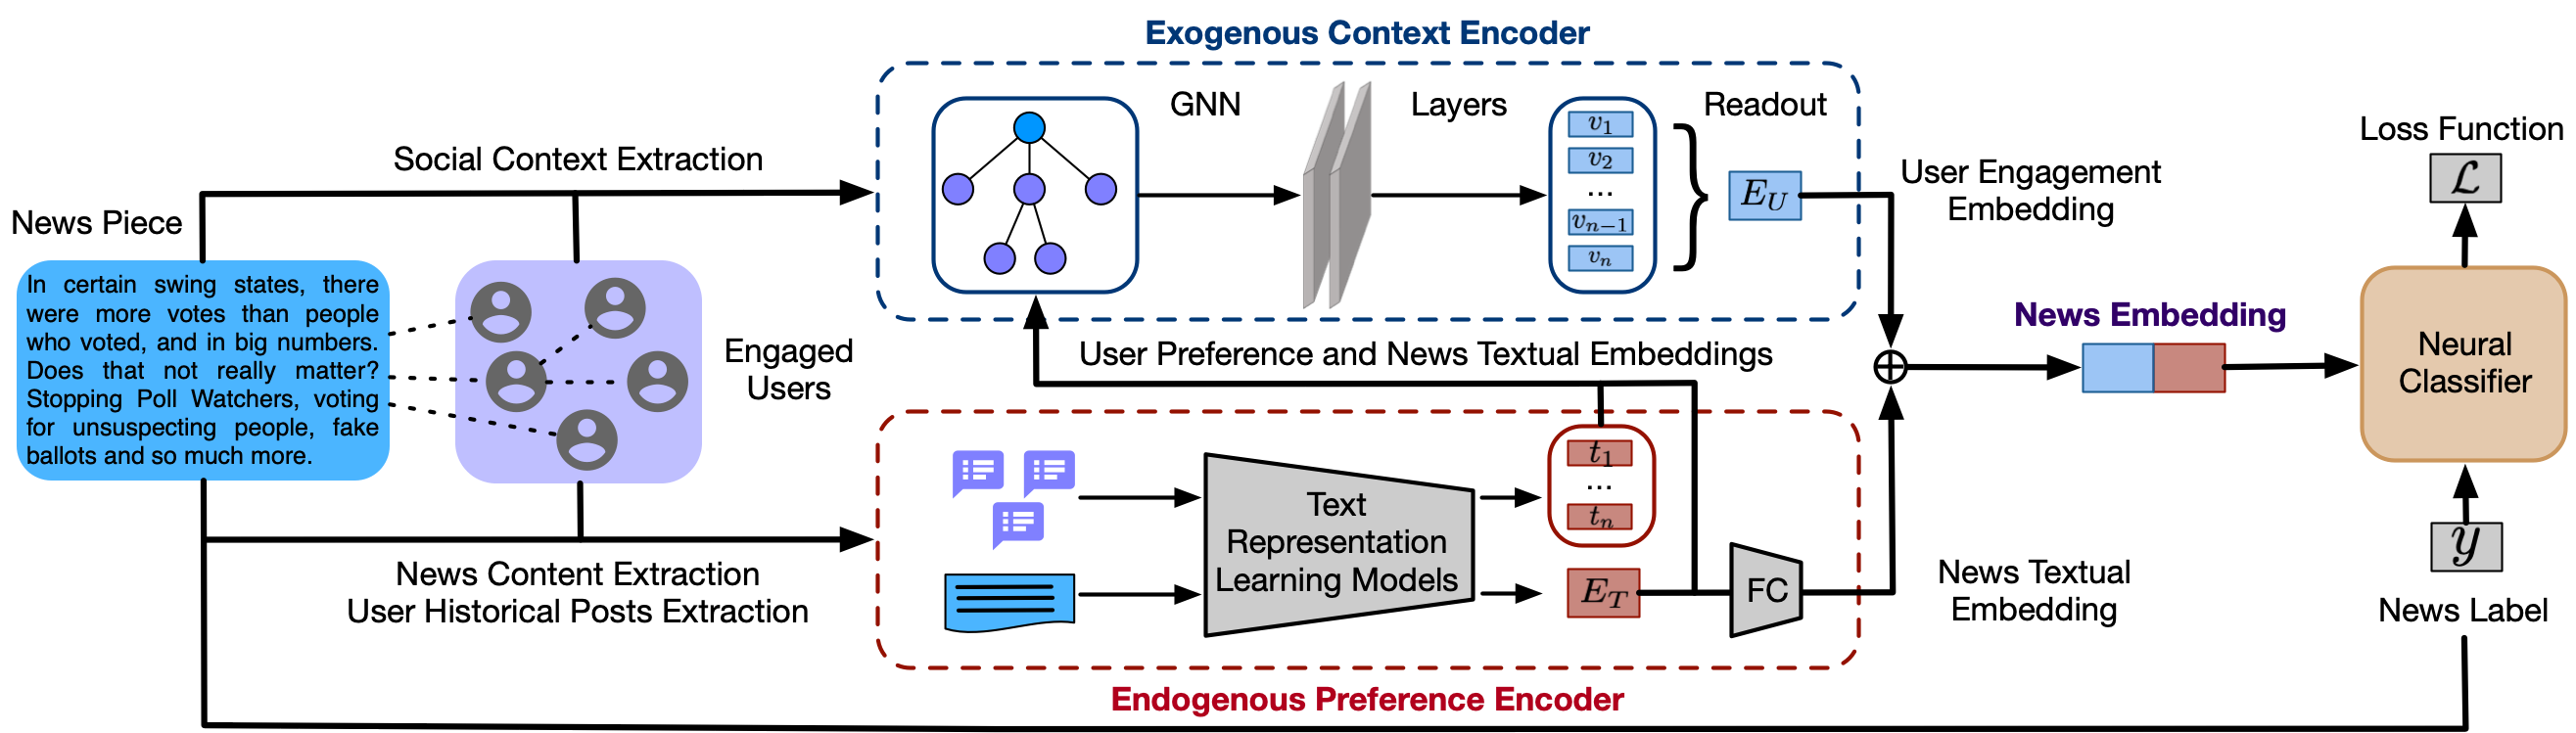
\includegraphics[scale=0.33]{UPFDFramework.png}
    \caption[UPFD Framework.]{The framework of UPFD. Figure obtained from~\parencite{UPFD_Dataset_Shu}}
    \label{fig:UPFD_Framework}
\end{figure}
\textbf{Endogenous preference encoding} deals with users' historical posts and news content using the news content and social engagement data in FakeNewsNet. With social engagement data, the authors collect 200 historical tweets of each user who have retweeted the news in FakeNewsNet. Summing up to almost 20 million tweets, this collection procedure of historical tweets for each FakeNewsNet news instance is as follows~\parencite{UPFD_Dataset_Shu}:
\begin{itemize}
    \item Collect user ids who have retweeted.
    \item For each user, collect the 200 most recent tweets.
    \item For inaccessible (suspended or deleted) users, use randomly sampled tweets from accessible users who engage in the same news piece. This step also increases the effectiveness of the exogenous encoder.
    \item  Finally, remove special characters such as "@" and URLs before applying textual techniques.
\end{itemize}
Now that we have news content and users' historical information, we encode these texts using text representation learning techniques. Still following~\cite{UPFD_Dataset_Shu}, the authors define two different settings for creating endogenous preference encoding. The first setting, \emph{spacy}, deals with obtaining the representation of users' historical data and news content with spaCy~\parencite{SpaCy_Honnibal} pretrained 300-dimensional vectors for 680K words. For each user's historical post (and similarly for each news piece), if a word appears in the text, we include the vector for that word for the final calculation in which all included vectors are averaged. As a result, we obtain a 300-dimensional vector for each user's historical information and news piece. The second setting, \emph{bert}, uses the BERT-Large model to encode news and historical user data. Using bert-as-a-service~\parencite{BertAsAService_Xiao}, the authors encode the news content with a maximum input sequence length of 768. The authors opt for a different setting to encode historical information since 200 tweets cannot be processed as a single document due to BERT's maximum input sequence length limitation of 768. It is important to note that the paper of UPFD~\parencite{UPFD_Dataset_Shu} states the maximum input sequence length as 512. However, in the dataset itself, the maximum sequence length is 768~\parencite{UPFD_PyGTeam}. Keeping in mind that tweets are usually short texts compared to news pieces, the authors use a maximum input sequence length of 16 for each historical tweet, then average all 200 tweets to obtain the final representation of users' historical data. This representation is of the same dimension as the root news node. Note that these text representation vectors are node features of a hierarchical tree-structured graph whose root node represents the news content, and the children of the root node represent the users who have retweeted.\\
\textbf{Exogenous context extraction} uses retweet information to build the previously mentioned hierarchical tree. The authors adopt a similar procedure used by~\citeauthor{GraphNeuralNetworksWithContinualLearningFakeNewsDetection_Han} (\citeyear{GraphNeuralNetworksWithContinualLearningFakeNewsDetection_Han}),\citeauthor{GeometricDeepLearningOnGraphsAndManifolds_Monti} (\citeyear{GeometricDeepLearningOnGraphsAndManifolds_Monti}), and \citeauthor{HierarchicalPropagationNetworksForFND_Shu} (\citeyear{HierarchicalPropagationNetworksForFND_Shu}). In detail, the authors define a news piece as $v_1$ and the set of users who retweeted $v_1$ as $\{v_2, \dots , v_n\}$ ordered by time. The rules are defined for this process to cover edge cases as well:
\begin{itemize}
    \item Estimate that a news piece propagates to user $v_i$ from user $v_j$ with the latest timestamp if any user from the set $\{v_j | j\in \{2, \dots, n\}\setminus \{i\}\}$ retweeted the news piece before the user $v_i$. This conservative assumption is based on the fact that the latest tweets are presented to the user first in the Twitter app~\parencite{UPFD_Dataset_Shu}.
    \item If user $v_i$ does not follow any users in the set $\{v_1, \dots, v_n \} \setminus {i}$, i.e., all retweeters and the news source except the user itself, the authors approximate the spreader of that news piece to the user $v_i$ as the user with most followers in the set. This approximation is based on the phenomenon that the tweets from accounts with more followers have a higher probability of being retweeted or viewed.
\end{itemize}
After this procedure, we have our hierarchical tree for each piece of news obtained from FakeNewsNet, which employs two sources: Politifact and Gossipcop. Thus, we evaluate these datasets separately within UPFD. The distribution of the instances with respect to train/validation/test split and label is provided in Fig.~\ref{fig:UPFD_Dataset_Visualization}.\\
\begin{figure}
    \subfloat[UPFD-Gossipcop]{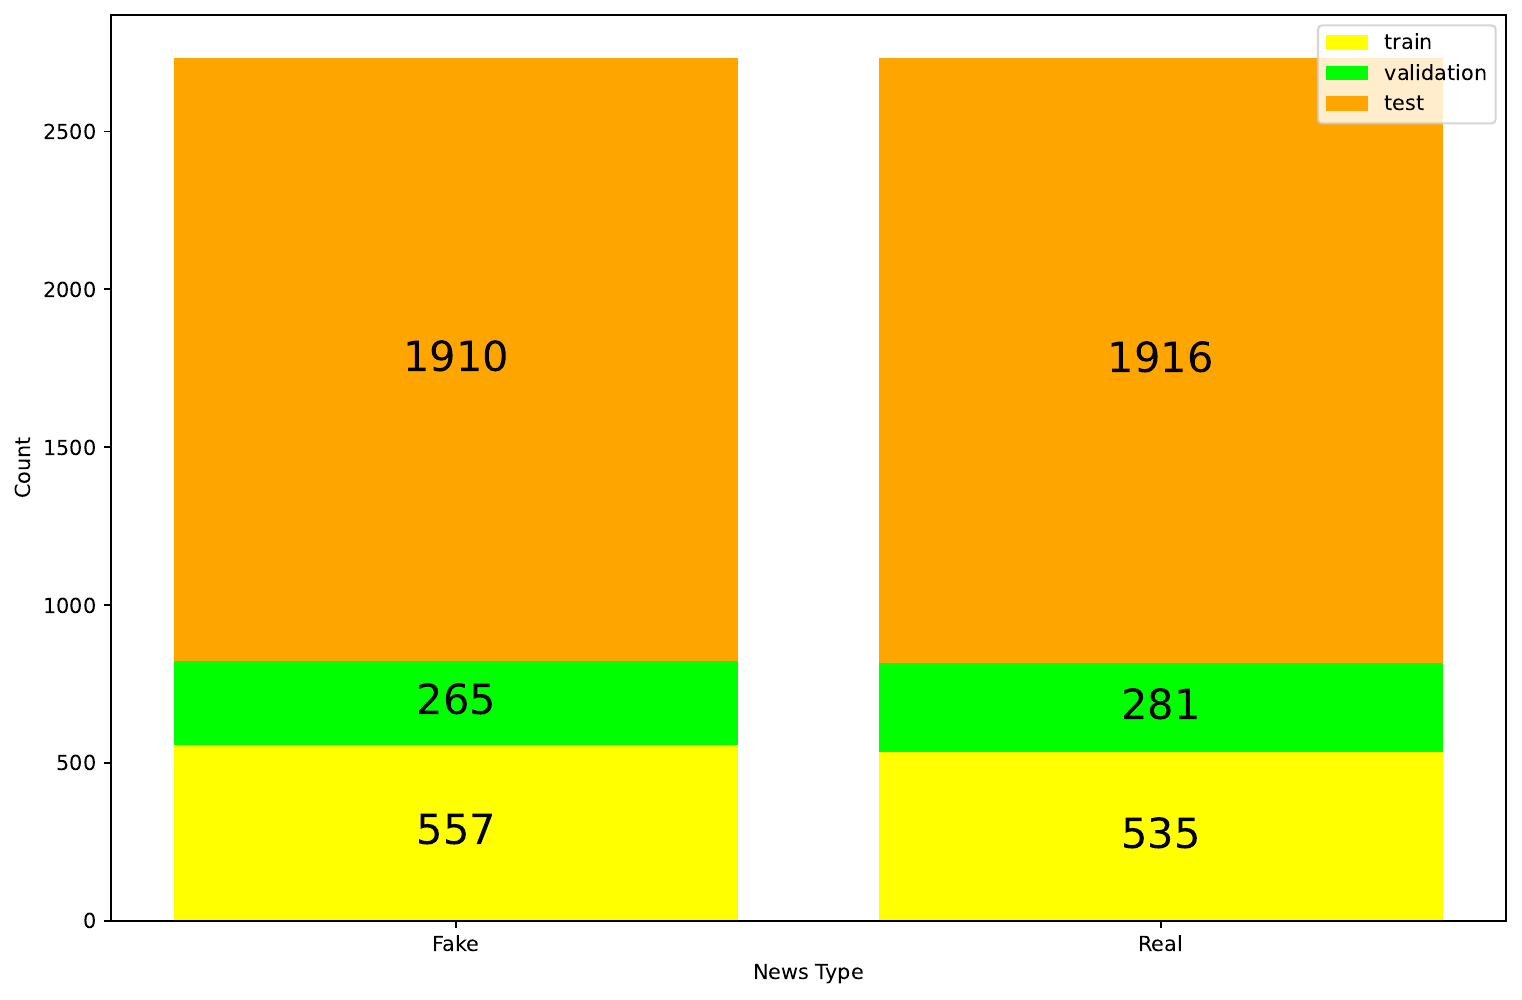
\includegraphics[width=0.45\textwidth]{GOS_DatasetDistrByLabelAndSplit.png}}
    \hfill
    \subfloat[UPFD-Politifact]{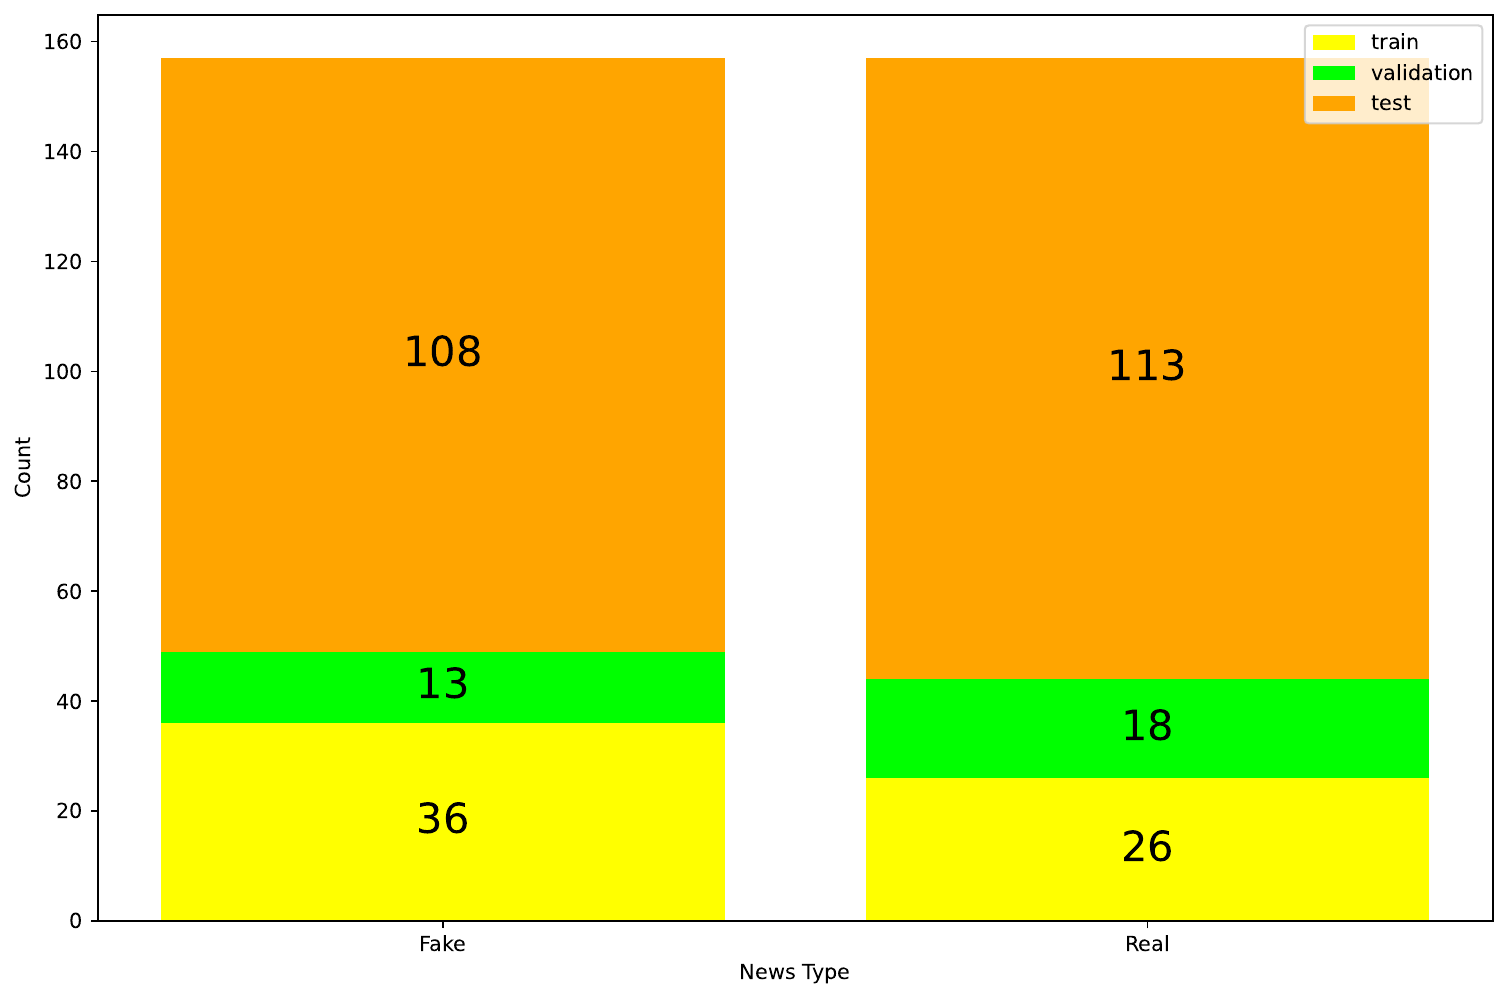
\includegraphics[width=0.45\textwidth]{POL_DatasetDistrByLabelAndSplit.png}}
    \caption[UPFD dataset distribution by label and split.]{UPFD dataset distribution by label and split (train: 20\%, val: 10\%, test: 70\%).}
    \label{fig:UPFD_Dataset_Visualization}
\end{figure}
\textbf{Information fusion} is achieved via GNNs. As discussed in~\ref{subsec:mixedApproaches_GraphNeuralNetworks}, GNNs can encode graphs by maintaining the node features and structural information. From this point on, we need to utilize the models we introduced with a classification setting. Classification is done for each graph representing the diffusion tree of the news piece~\parencite{UPFD_Dataset_Shu}. We adopted two models from this work's ablation study, the first one is based on GraphSAGE~\parencite{GraphSAGE_Hamilton}, and classification is handled with an FCN. We use BERT as the encoder since the best performance is obtained via that, according to the experiments by~\citeauthor{UPFD_Dataset_Shu} (\citeyear{UPFD_Dataset_Shu}) and the experiments we conducted. We call this model the UPFD classifier. It is illustrated in Fig~\ref{fig:UPFDClassifierArchitecture}.\\
\begin{figure}
    \centering
    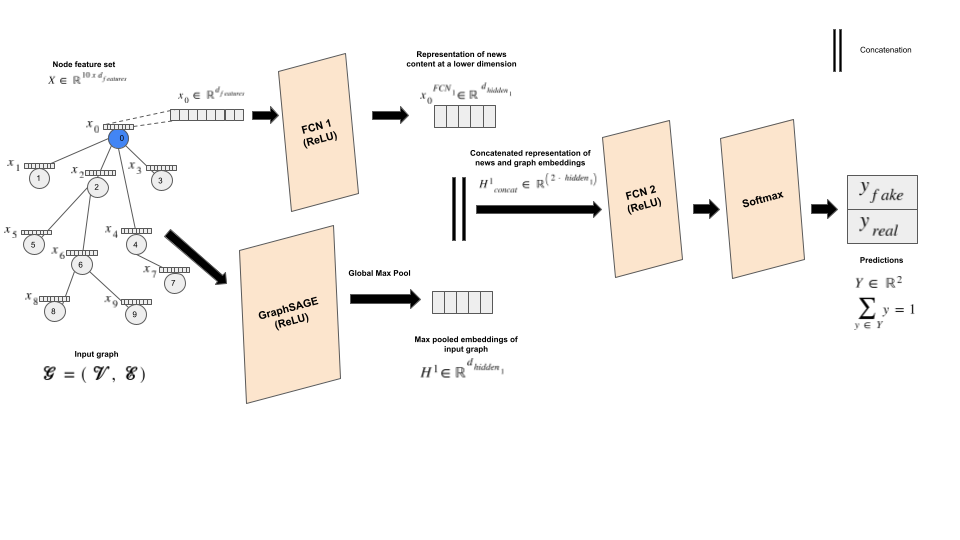
\includegraphics[scale=0.43]{UPFDClassifierArchitecture}
    \caption[The UPFD classifier model pipeline.]{The UPFD classifier model pipeline. We used an example input graph with 10 nodes. $d_{hidden_1} = 128$ stands for hidden layer dimension of FCN 1, accordingly, $d_{hidden_2} = 128$ for the hidden dimension of FCN 2, and $d_{features} = 768$ for feature dimension.}
    \label{fig:UPFDClassifierArchitecture}
\end{figure}
After obtaining the graph encodings, the authors suggest concatenating a representation of news content with graph embeddings. More precisely, the feature vector of the root node is fed to an FCN to obtain a lower-dimensional representation which is then concatenated with graph embeddings. The concatenated vector is then fed to another FCN and the softmax layer for classification. With the setting illustrated in Fig~\ref{fig:UPFDClassifierArchitecture}, the optimizer as Adam with default $\beta_1$ and $\beta_2$ and hyperparameters provided in Table~\ref{tab:UPFDClassifier_Hyperparameters}, we obtain 95.49\% and 83.16\% accuracy from the UPFD-Gossipcop and UPFD-Politifact datasets, averaged by ten runs, respectively. All other statistics are provided in Table~\ref{tab:UPFDClassifier_Results}.\\
\begin{table}
    \centering
    \begin{tabular}{|l|l|}
        \hline
        Activation function & ReLU~\parencite{ReLU_Nair} \\
        \hline
        Batch size          & 128                        \\
        \hline
        Epochs              & 35                         \\
        \hline
        Learning rate       & 0.01                       \\
        \hline
        Hidden layer 1 size & 128                        \\
        \hline
        Hidden layer 2 size & 128                        \\
        \hline
        Weight decay        & 0.01                       \\
        \hline
    \end{tabular}
    \caption[Hyperparameters of the UPFD classifier.]{Hyperparameters of the UPFD classifier.}
    \label{tab:UPFDClassifier_Hyperparameters}
\end{table}
\begin{table}
    \centering
    \begin{tabular}{c | c | c | c | c}
        \textbf{Dataset} & \textbf{Accuracy} & \textbf{Precision} & \textbf{Recall} & \textbf{F1 score} \\
        \hline
        UPFD-Gossipcop   & 95.49\%           & 94.95\%            & 96.17\%         & 95.50\%           \\
        \hline
        UPFD-Politifact  & 83.16\%           & 84.05\%            & 82.19\%         & 83.25\%           \\
    \end{tabular}
    \caption[The UPFD classifier performance metrics averaged over 10 runs.]{The UPFD classifier performance metrics averaged over 10 runs.}
    \label{tab:UPFDClassifier_Results}
\end{table}
From the model architecture, we can easily see that the UPFD classifier's social context part is propagation-based and utilize a homogeneous network. On the other hand, the news content part is unknown, but it can be uncovered using explanation techniques for GNNs. Before we explain the UPFD classifier, we outline the features of UPFD.\\
To recap, the UPFD is constructed with the news pieces and social context data obtained from FakeNewsNet~\parencite{FakeNewsNet_Shu}. \citeauthor{HierarchicalPropagationNetworksForFND_Shu} (\citeyear{HierarchicalPropagationNetworksForFND_Shu}) utilize the data from FakeNewsNet to create two levels of propagation networks: \emph{macro-level} and \emph{micro-level}. For each level,~\citeauthor{HierarchicalPropagationNetworksForFND_Shu} (\citeyear{HierarchicalPropagationNetworksForFND_Shu}) define and statistically test the significance of a set of features. We want to see if some of those features are adopted by the UPFD classifier. Briefly, macro-level networks are constructed to track the diffusion of a news piece via retweets, whereas micro-level propagation networks are built using replies to retweets. UPFD is the macro-level propagation network. Thus our focus is on the features of the macro-level propagation network.\\
The features are macro-level propagation networks are categorized into two: \emph{structural} and \emph{temporal}. Structural features capture the patterns in the global dissemination of a news piece~\parencite{HierarchicalPropagationNetworksForFND_Shu}. These features include:
\begin{itemize}
    \item ($SF_1$) \emph{Tree Depth}: Indicates how far the news piece has spread through the propagation network~\parencite{HierarchicalPropagationNetworksForFND_Shu}.
    \item ($SF_2$) \emph{Number of nodes in macro-network}: Indicates how many users have shared the news piece~\parencite{HierarchicalPropagationNetworksForFND_Shu}.
    \item ($SF_3$) \emph{Maximum outdegree}: Helps reveal the tweet/retweet with the most influence in the propagation network~\parencite{HierarchicalPropagationNetworksForFND_Shu}.
    \item ($SF_4$) \emph{Number of cascades}: The number of tweets that post the original news article~\parencite{HierarchicalPropagationNetworksForFND_Shu}.
    \item ($SF_5$) \emph{Depth of node with maximum outdegree}: Indicates steps of propagation required for a news piece to be retweeted by an influential user (node) whose post is retweeted by more users than any other users' retweet~\parencite{HierarchicalPropagationNetworksForFND_Shu}.
    \item ($SF_6$) \emph{Number of cascades with retweets}: Indicates the number of tweets that shared the original news article and retweeted at least once~\parencite{HierarchicalPropagationNetworksForFND_Shu}.
    \item ($SF_7$) \emph{Fraction of cascades with retweets}: Corresponds to $SF_6 / SF_4$~\parencite{HierarchicalPropagationNetworksForFND_Shu}.
    \item ($SF_8$) \emph{Number of bot users retweeting}: Captures the number of bot users that retweeted that news piece~\parencite{HierarchicalPropagationNetworksForFND_Shu}.
    \item ($SF_9$) \emph{Fraction of bot users retweeting}: Corresponds to $SF_8 / SF_2$~\parencite{HierarchicalPropagationNetworksForFND_Shu}.
\end{itemize}
First of all, the feature set is not restricted to these features. One can derive more features from this dataset. We
will investigate some of these features in order to understand whether we can capture similar features in our explanations.
We do not have access to the information of bot users in UPFD. Thus we drop the analysis of features $SF_8$ and $SF_9$. In addition, we did not analyze temporal features, as obtaining them from the explanation proved to be a long process. We now discuss which features' average values are found to be significant in the statistical tests conducted by~\citeauthor{HierarchicalPropagationNetworksForFND_Shu} (\citeyear{HierarchicalPropagationNetworksForFND_Shu}).\\
The first structural feature $SF_1$ is found to be consistently different for real and fake news instances in both datasets, under the statistical t-test~\parencite{HierarchicalPropagationNetworksForFND_Shu}. Concretely, this finding indicates that the tree depth of the fake news pieces is larger than that of real news pieces. Next, another simple feature $SF_2$ is also shown to be consistently different. Fake news instances have fewer nodes than real news instances. Although helpful, without additional information, this feature is too broad. Thus, we look at the next structural feature $SF_3$. It is found by~\citeauthor{HierarchicalPropagationNetworksForFND_Shu} (\citeyear{HierarchicalPropagationNetworksForFND_Shu}) that this feature is consistently different for fake and real news in Gossipcop under t-test. More precisely, it is found that the maximum outdegree is bigger in fake news instances of Gossipcop. Considering this observation, we now proceed to more complex features.\\
When we look at features that analyze more subtle properties of the dataset, such as $SF_5$ and $SF_7$, it is reported that these features are also consistently different for fake and real news instances from both datasets~\parencite{HierarchicalPropagationNetworksForFND_Shu}. According to the study, $SF_5$ is discovered to be deeper for fake news instances. The other feature $SF_7$ investigates how many of the first retweeters of the original post were retweeted. The t-test tells us that this value is different in real and fake news instances in both datasets. Specifically, the value of $SF_7$ is higher for fake news than for real news.\\
We have introduced the dataset and the model we have employed for FND in mixed approaches. We will analyze the model's behavior on the dataset. We adopt GNNExplainer~\parencite{GNNExplainer_Ying} as our explanation tool and try to uncover the patterns the model has learned. We shall also discuss some limitations we encountered while conducting these experiments.

\section{Explaining Graph Neural Networks}
\label{sec:ExplainingGNNs}
Except for GNNs, many neural networks can be explained using various tools, such as SHAP, LIME, and LRP, to name the most common ones. GNNs make their predictions by aggregating information from nodes, edges, and graph topology. There can be cases where an edge plays a significant role in the node prediction only if it is considered with another edge~\parencite{CNNsOnGraphsForLearningMolecularFingerprints_Duvenaud}. Therefore, we can not model separate contributions of node,
edge, and graph features in a linear manner.\\

\subsection{GNNExplainer}
\label{subsec:ExplainingGNNs_GNNExplainer}
GNNExplainer is a post-hoc model-agnostic explainer tool that aims to provide information about the effects of node features, edges, and graph structure on the prediction. More precisely, let us denote the node $v$'s computation graph as $\mathcal{G}_c(v)$, the binary adjacency matrix as $\mathcal{A}_c(v) \in \{0, 1\}^{n \times n}$ with $n$: the number of nodes, and the feature set as $X_c(v) = \{x_j|v_j \in \mathcal{G}_c(v)\}$. Then we say that a GNN model $f$ learns a conditional distribution $P_f(Y | \mathcal{G}_c, X_c)$ with $Y \in \{1, \dots, C\}$ as a random variable that stands for class probabilities of nodes. Then in probabilistic terms, the prediction is denoted as $\hat{y} = f(\mathcal{G}_c(v), X_c(v))$, which suggests that the prediction depends on three parts. Therefore, GNNExplainer takes into account the GNN model $f$, the graph information $\mathcal{G}_c(v)$, and the node features $X_c(v)$~\parencite{GNNExplainer_Ying}.\\
Simply put, GNNExplainer finds a subgraph $\mathcal{G}_S(v) \in \mathcal{G}_c(v)$ and node feature subset $X_S = \{x_j | v_j \in \mathcal{G}_S\}$ that are important for a given prediction $\hat{y}$. The subgraph that explains the prediction best is obtained by maximizing the \emph{mutual information} $MI$ between the prediction $Y$ and the pair of subgraph and subset of node features $(\mathcal{G}_S, X_S)$~\parencite{GNNExplainer_Ying}.
\begin{center}
    $\max\limits_{\mathcal{G}_S} MI(Y, \mathcal{G}_S, X_S) = H(Y) - H(Y|G=\mathcal{G}_S, X=X_S)$
\end{center}
where $H(Y)$ is the marginal entropy of $Y$ and is fixed for a trained GNN, and $H(Y|G=\mathcal{G}_S, X=X_S)$ stands for the conditional entropy. Since $H(Y)$ is fixed, the authors reformulate the objective function as a minimization function that looks for a subgraph $\mathcal{G}_S$ that minimizes the uncertainty of the GNN model $f$ while using a subset of node features $X_S$, thus maximizing the probability of $\hat{y}$. However, this formulation brings computation issues as large dense graphs can have massive amounts of candidate explaining subgraphs for a prediction $\hat{y}$. Thus, the authors enforce a constraint on the fractional adjacency matrix $A_S \in [0, 1]^{n \times n}$ of the subgraphs, which are now treated as random variables $\mathcal{G}_S \sim \mathcal{G}$. With convexity assumption and upper-bound from Jensen's inequality, the minimization problem is rewritten as~\parencite{GNNExplainer_Ying},
\begin{center}
    $\min\limits_{\mathcal{G}} = H(Y | G = \mathbb{E}_{\mathcal{G}} [\mathcal{G}_S, X = X_S])$.
\end{center}
Finally, to estimate $\mathbb{E}_{\mathcal{G}}$, the authors employ mean-field variational approximation and decompose $\mathcal{G}$ into a multivariate Bernoulli distribution. This allows estimating the expectation in terms of the mean-field approximation. Thus, obtaining $A_S$ whose $(i, j)$-th element denotes the expectation of the existence of the edge $(v_i, v_j)$. The final objective is defined as,
\begin{center}
    $\min\limits_M - \sum\limits_{c=1}^C \mathbb{1}[y = c] \;\;log(P_f (Y=y \;|\; \mathcal{G} = A_S \bigodot \sigma(M), X = X_S))$
\end{center}
where $M \in \mathbb{R}^{n \times n}$ is the mask to learn, $\bigodot$ is element-wise multiplication, and $\sigma$ is
the mapping function of the mask to values to interval $[0, 1]^{n \times n}$~\parencite{GNNExplainer_Ying}. For large graphs, however, a threshold might be required to remove low values in the mask. We will propose two approaches to effectively
handle this only for explanations of the UPFD classifier~\parencite{GNNExplainer_Ying}.\\
Besides the edge mask $M$, as mentioned previously, GNNExplainer also learns a node mask $F \in \{0, 1\}^d_{features}$ through a binary feature selector that is learned by maximizing $MI$ in the first equation. Formally, the explanation $(\mathcal{G}_S, X_S)$ is optimized together to maximize $MI$:
\begin{center}
    $\max\limits_{\mathcal{G}_S, F} \;\; MI (Y, (\mathcal{G}_S, F)) = H(Y) - H(Y \;|\; \mathcal{G} = \mathcal{G}_S,\; X = X_S^F)$
\end{center}
where $X_S^F = \{x_j^F|v_j \in \mathcal{G}_S\}$ and $x_j^F = [x_{j, t_1}, \dots, x_{j, t_k}]$ for
$F_{t_i} = 1$ denotes the node features that are not masked out by F~\parencite{GNNExplainer_Ying}. So far, the
explanation method is defined for the node classification setting. However, when the task is at the graph-level, the method needs to be extended. \citeauthor{GNNExplainer_Ying} (\citeyear{GNNExplainer_Ying}) suggest unionizing the adjacency matrices $A_S$ for all nodes in the graph to be explained. The aggregation of node embeddings, however, restricts the explanation to a subset, where the resulting subgraph must be connected. Thus, the threshold for the edge mask is set to a very low value or zero. This allows for a larger connected subgraph as an explanation~\parencite{GNNExplainer_Ying}.\\


\subsection{Explainability of UPFD Classifier}
\label{subsec:ExplaniningGNNs_ExplainingUPFDClassifier}
In Section~\ref{sec:mixedApproaches}, we have introduced the UPFD classifier, a GNN that uses GraphSAGE~\parencite{GraphSAGE_Hamilton} as the graph encoder, two FCNs, and softmax for the classification of news propagation trees. We now investigate the mixed model's behavior on the UPFD-Politifact dataset by employing GNNExplainer. Note that this model was trained only on the UPFD-Politifact dataset; thus, data in UPFD-Gossipcop is unseen to this model. The explanations we obtain for our classifier on the UPFD-Politifact dataset might provide us with useful information that allows us to understand the model's reasoning.\\
First, to clarify how the explanations should be interpreted, let us consider an example where we obtain a single explanation $(\mathcal{G}_S, X_S)$ for a news diffusion tree. We interpret the edge masks $M$ of $\mathcal{G}_S$ as the importance scores of edges between nodes. Therefore, an edge $(v_i, v_j)$ with a mask value $m_{ij}$ lower than a fixed $threshold$ will be dropped. After the $threshold$ is applied, if a node $v_i$ is not connected to the largest connected subgraph, it will not be included in the visualization of the explanation. \\
\begin{figure}
    \centering
    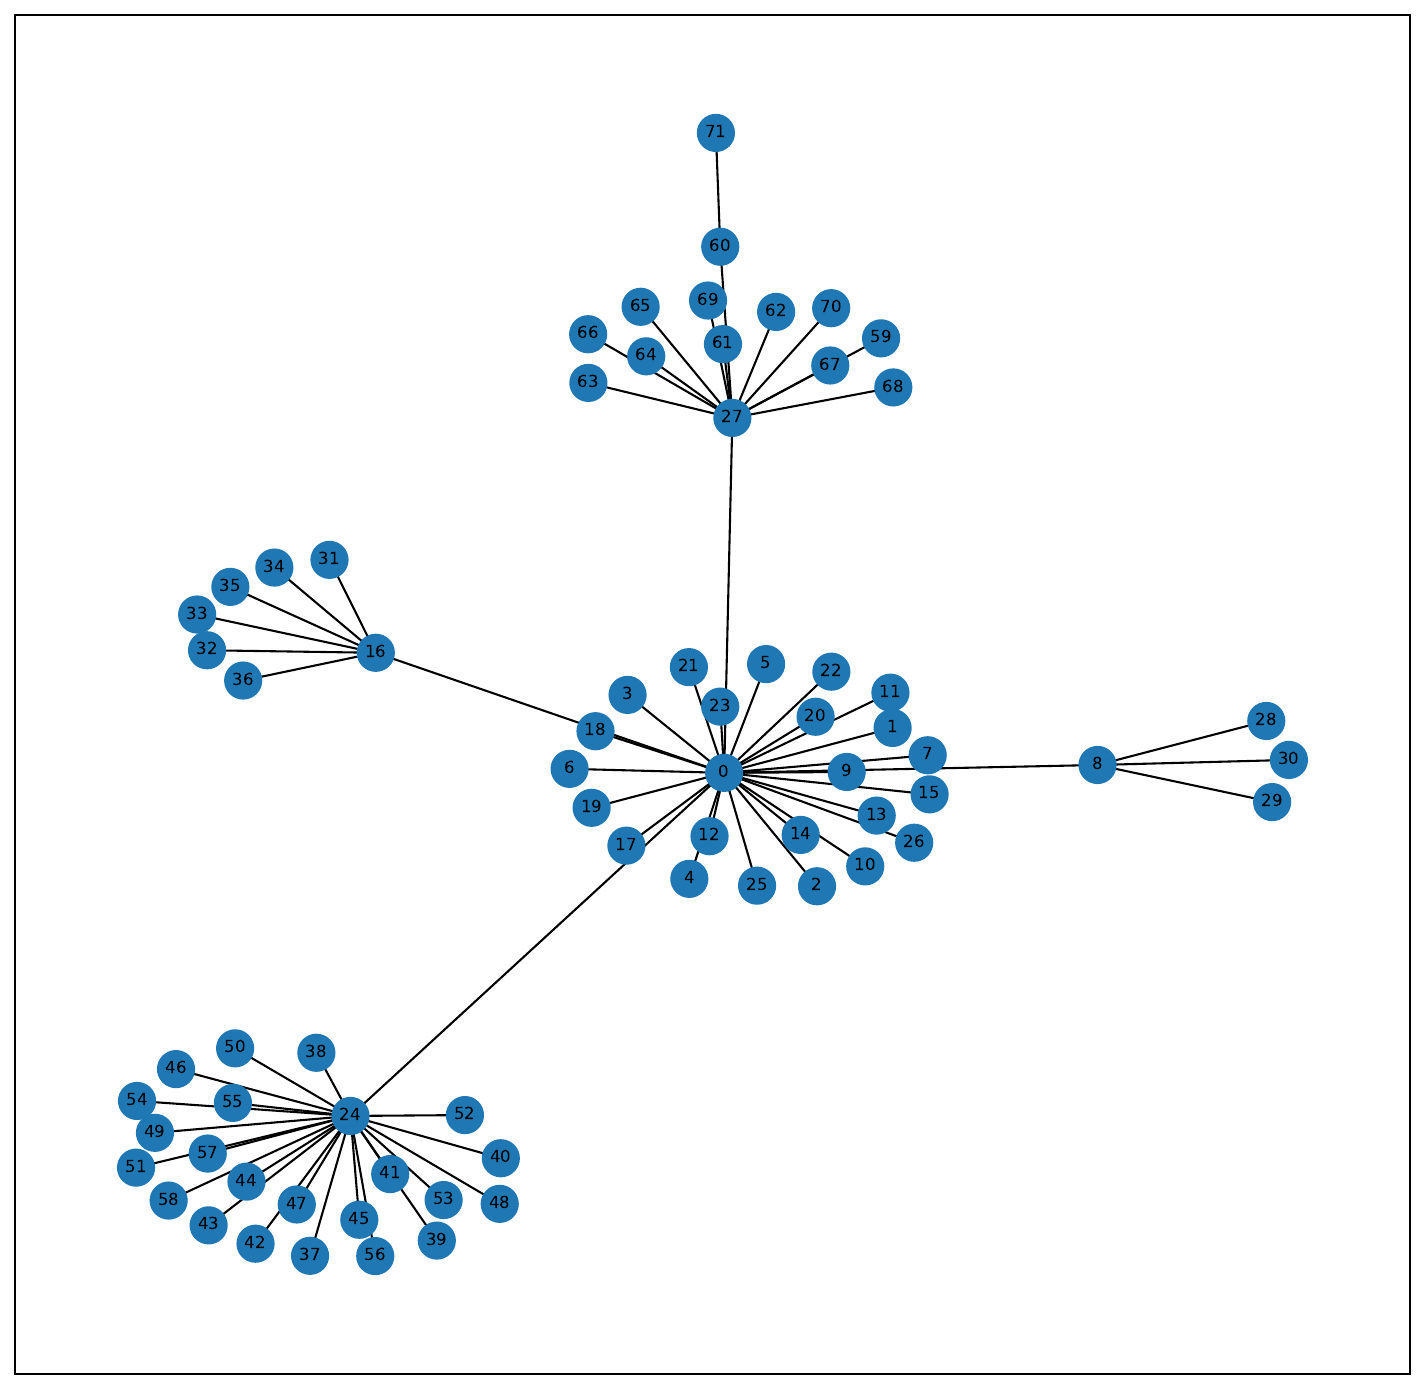
\includegraphics[scale=0.45]{EchoChamberExample1}
    \caption[Echo chamber example from the UPFD-Politifact dataset.]{A fake news instance in the UPFD-Politifact dataset that exhibits echo chamber behavior. $0$-th node represents the root node with news embeddings. We will refer to this fake news example as the \emph{echo chamber example}.}
    \label{fig:echoChamberExample1}
\end{figure}
We examine whether our classifier learned a similar intuition that we discussed in~\ref{subsec:fakeNewsDetection_fakeNews}. Recall that echo chambers are one of the significant reasons that fake news pieces spread. We analyze an example from the train split of the UPFD-Politifact dataset, some of whose cascade nodes exhibit echo chamber structures. To be precise, there is no clear definition of echo chambers in the context of diffusion trees. For the echo example in Fig.~\ref{fig:echoChamberExample1}, we assume that any cascade node with more than two child nodes, each of which do not have children, has an echo chamber.\\
In the echo chamber example in Fig.~\ref{fig:echoChamberExample1}, we observe some echo chambers created by cascade nodes $24$, $27$, $16$, and $8$ from biggest to smallest, respectively. We look for features introduced in~\ref{subsec:mixedApproaches_DatasetAndModel} that are captured by the UPFD classifier. First, let us observe the explaining subgraph $\mathcal{G}_S$ in Fig~\ref{fig:EchoChamberExample1Explanation_no_threshold} for the echo chamber example.\\
\begin{figure}
    \centering
    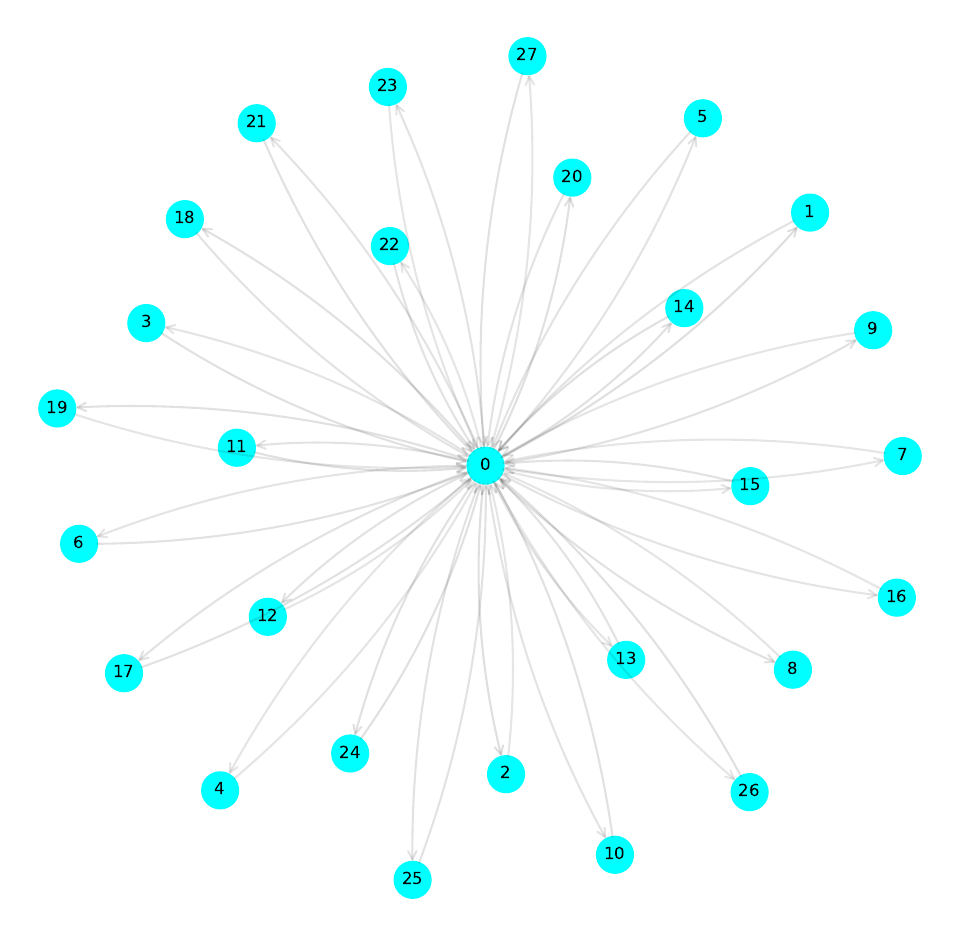
\includegraphics[scale=0.45]{EchoChamberExample1Explanation_no_threshold.png}
    \caption[Echo chamber example explanation for root node.]{The explanation provided for the UPFD classifier and the echo chamber example for its root node. This instance was predicted as fake news with a probability of $0.9912$. Contains 28 nodes.}
    \label{fig:EchoChamberExample1Explanation_no_threshold}
\end{figure}
Even though UPFD has undirected edges, we have obtained an explanation with bidirectional directed edges. Recall that undirected edges are interpreted as bidirectional edges. This is why GNNExplainer provided us with two edges per node pair. Additionally, there exist self-loops for each node, but those are not included in the visualization. Self-loops are edges from and to the same node $(v_i, v_i)$. The edge mask values for edges indicate the importance of the messages passed between two nodes. The transparency of the edges is an indicator of the magnitude of the edge mask value. However, this can not be clearly observed in this example.\\
On the other hand, when we inspect the node feature mask $F$, we can understand which features are deemed important by the UPFD classifier for a given node. We are particularly interested in the root node and the node feature mask associated with it. Since the root node consists of news content embeddings, intuitively, we can consider the root node feature mask as the importance scores of news content embeddings or tokens. However, we were not able to utilize node feature masks due to (i) the time needed to download the FakeNewsNet~\parencite{FakeNewsNet_Shu} (around 80\% was completed in over two months), whose news content and social context data were utilized in UPFD, (ii) insufficient information from~\citeauthor{UPFD_Dataset_Shu} (\citeyear{UPFD_Dataset_Shu}) to reproduce the UPFD framework, (iii) large maximum input sequence (768) for BERT model to process the news content on a local computer. Thus, we continue our analysis without considering the node feature mask. \\
\textbf{Interpreting the Explanation.} According to the explaining subgraph, the UPFD classifier thinks that the cascades are the most important nodes for the prediction of fake for this instance. If we only consider the echo chamber effect, we would expect higher edge mask values for the edges of the cascade nodes $v_8$, $v_{16}$, $v_{24}$, and $v_{27}$. Accordingly, we observe larger importance scores on edges that connect these nodes to the root node. The edge $(v_0, v_{13})$ was assigned the highest edge mask value with $0.1371$. The edges $(v_0, v_8)$, $(v_0, v_{16})$, $(v_0, v_{24})$, and $(v_0, v_{27})$ were assigned $0.1081$, $0.0951$, $0.1222$, and $0.1181$, respectively.  While the reasons behind the maximal importance score assignment to the edge $(v_0, v_{13})$ remain unclear, we observe that the biggest echo chamber's connection to the root node has a high edge mask value, which suggests that the UPFD classifier might be utilizing the echo chamber effect with success for prediction. However, we need to observe similar behaviors in other fake news instances that house echo chambers.\\
We also examined five edges with the highest edge mask values to understand which edges are important for the UPFD classifier. Before we proceed, it should be noted that the subgraph generation does not directly take into account where the maximal edge mask values reside. Instead, it tries to capture the biggest subgraph with the highest mutual information between the original graph and the subgraph with respect to the prediction. Hence, some edges we will analyze might not be in the explaining subgraph.\\
\textbf{Edge Mask Analysis.} Proceeding our analysis for the five largest values in the edge mask provided by GNNExplainer, we observed that the second highest value belongs to the edge $(v_{24}, v_{41})$, i.e., an echo chamber connection. The third one belongs to a self-loop $(v_{44}, v_{44})$, and the fourth one is for the edge $(v_{44}, v_{24})$. We can interpret the edge mask value for the self-loop as the significance that the UPFD classifier puts on node $v_{44}$. The edge mask value for edge $(v_{44}, v_{24})$ confirms our interpretation for node $v_{44}$ because this is the first instance of an important edge that is directed from a retweeter to its source. Thus, the user $v_{44}$ and their historical data should be investigated for further insights. Also, one can look for the same user in the other fake news instances to understand this user's involvement. The fifth-largest edge mask value is assigned to the edge $(v_{27}, v_{62})$, which is another propagation edge in an echo chamber. The distribution of the edge mask values is given in Fig.~\ref{fig:EchoChamber1SubgraphEdgeMaskDistribution}.\\
% \begin{figure}
%     \centering
%     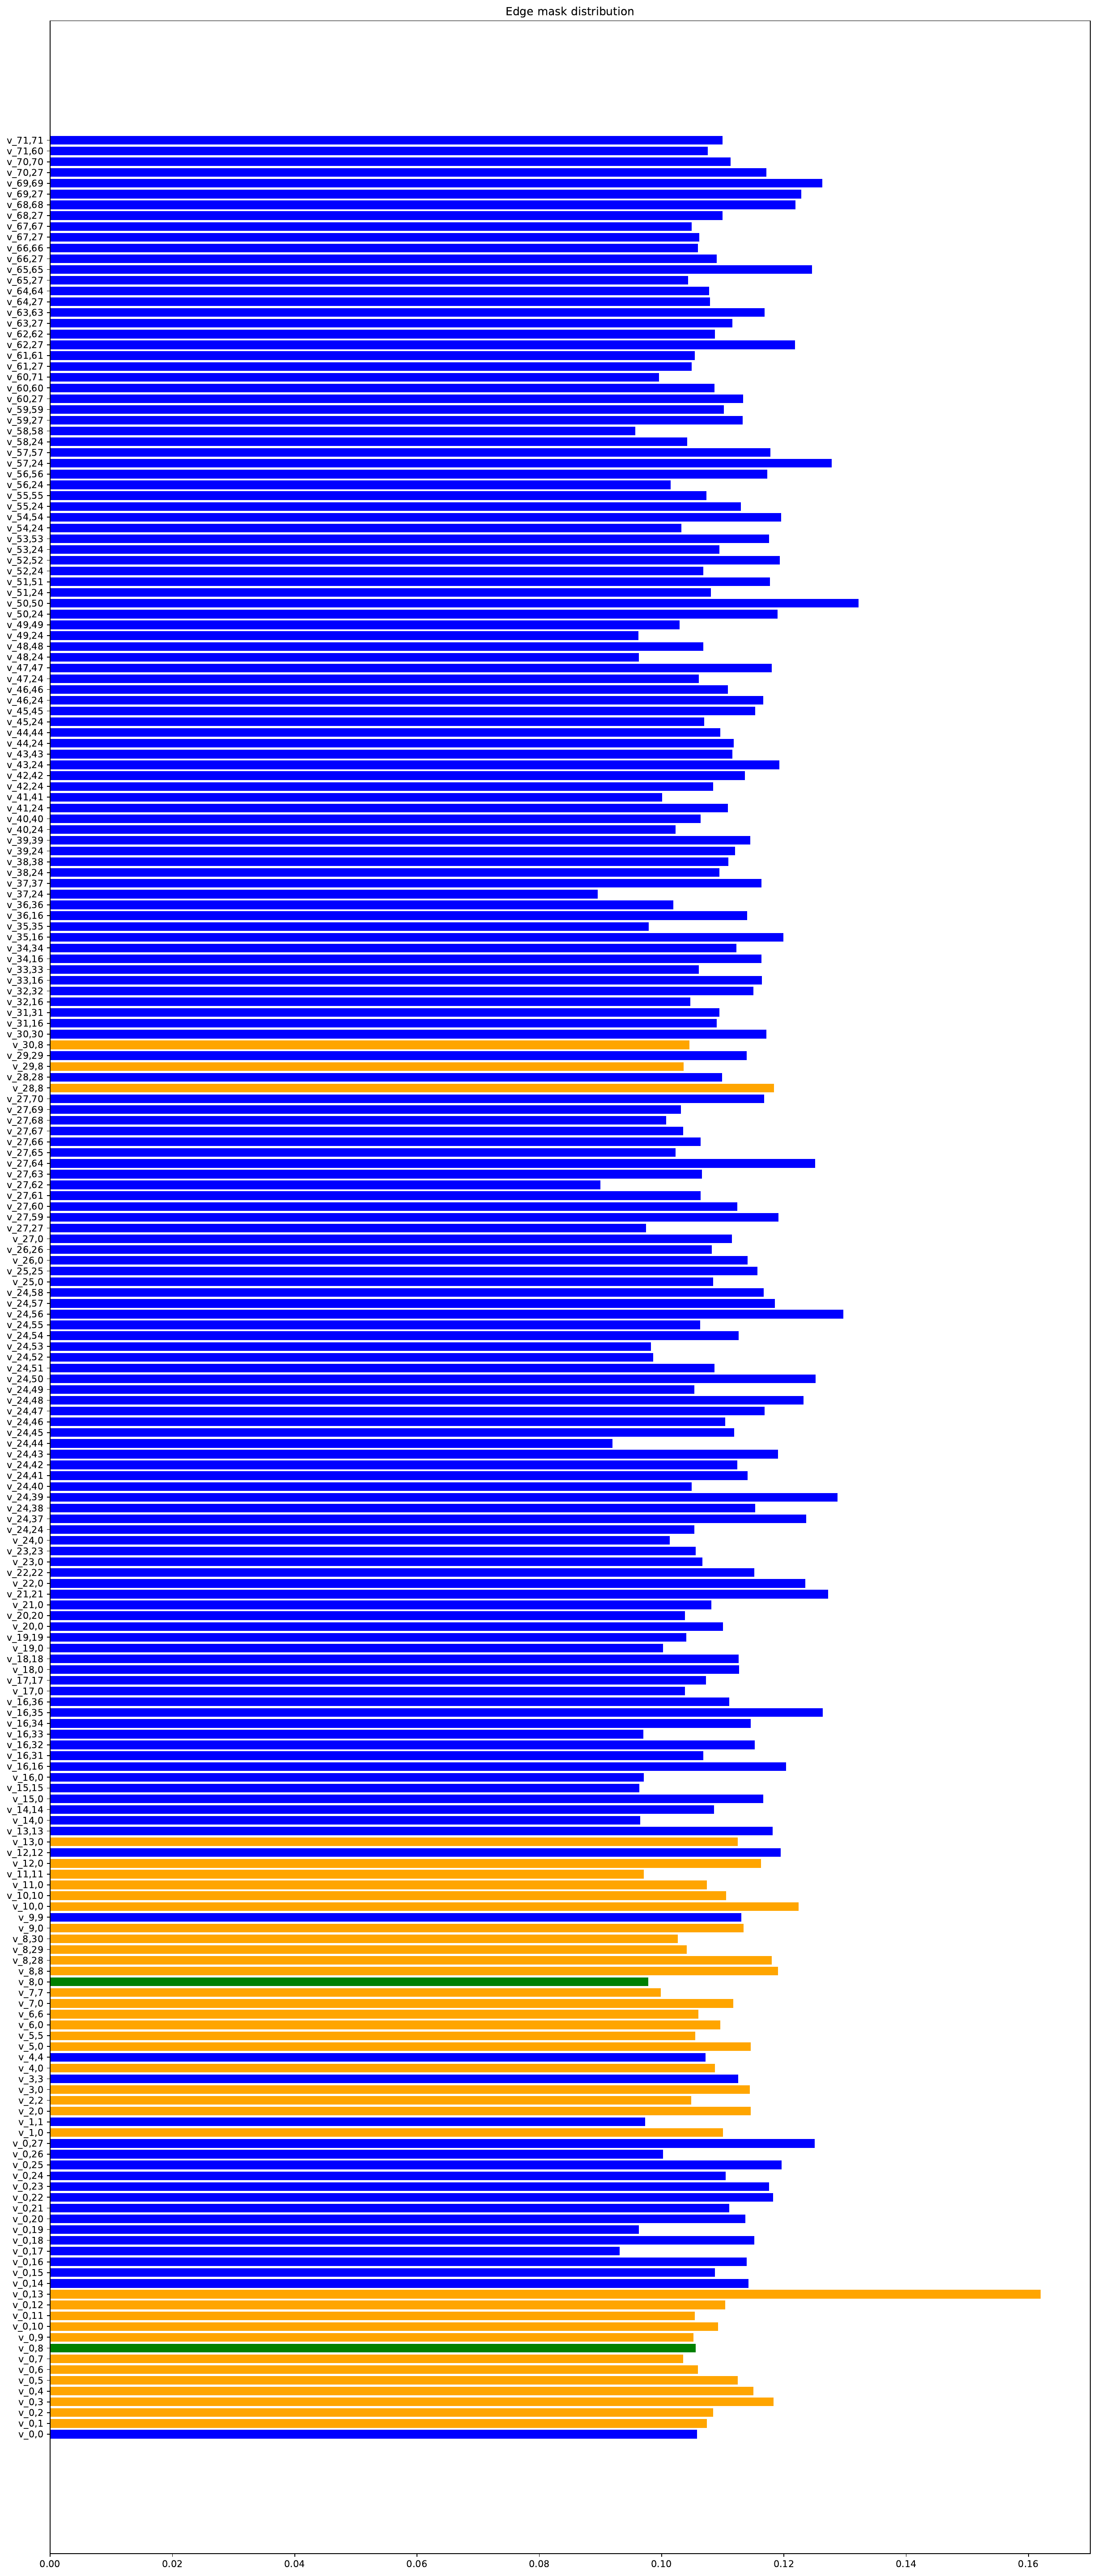
\includegraphics[scale=0.15]{EchoChamber1EdgeMaskDistribution.png}
%     \caption[Edge mask distribution of the input graph provided for echo chamber example explanation.]{Edge mask distribution of the input graph provided for echo chamber example explanation. The orange bars represent the edge mask values of the edges included in the subgraph explanation. Green bars indicate edges with the same characteristic as orange bars, but these edges are also connections to echo chambers.}
%     \label{fig:EchoChamber1EdgeMaskDistribution}
% \end{figure}
\begin{figure}
    \centering
    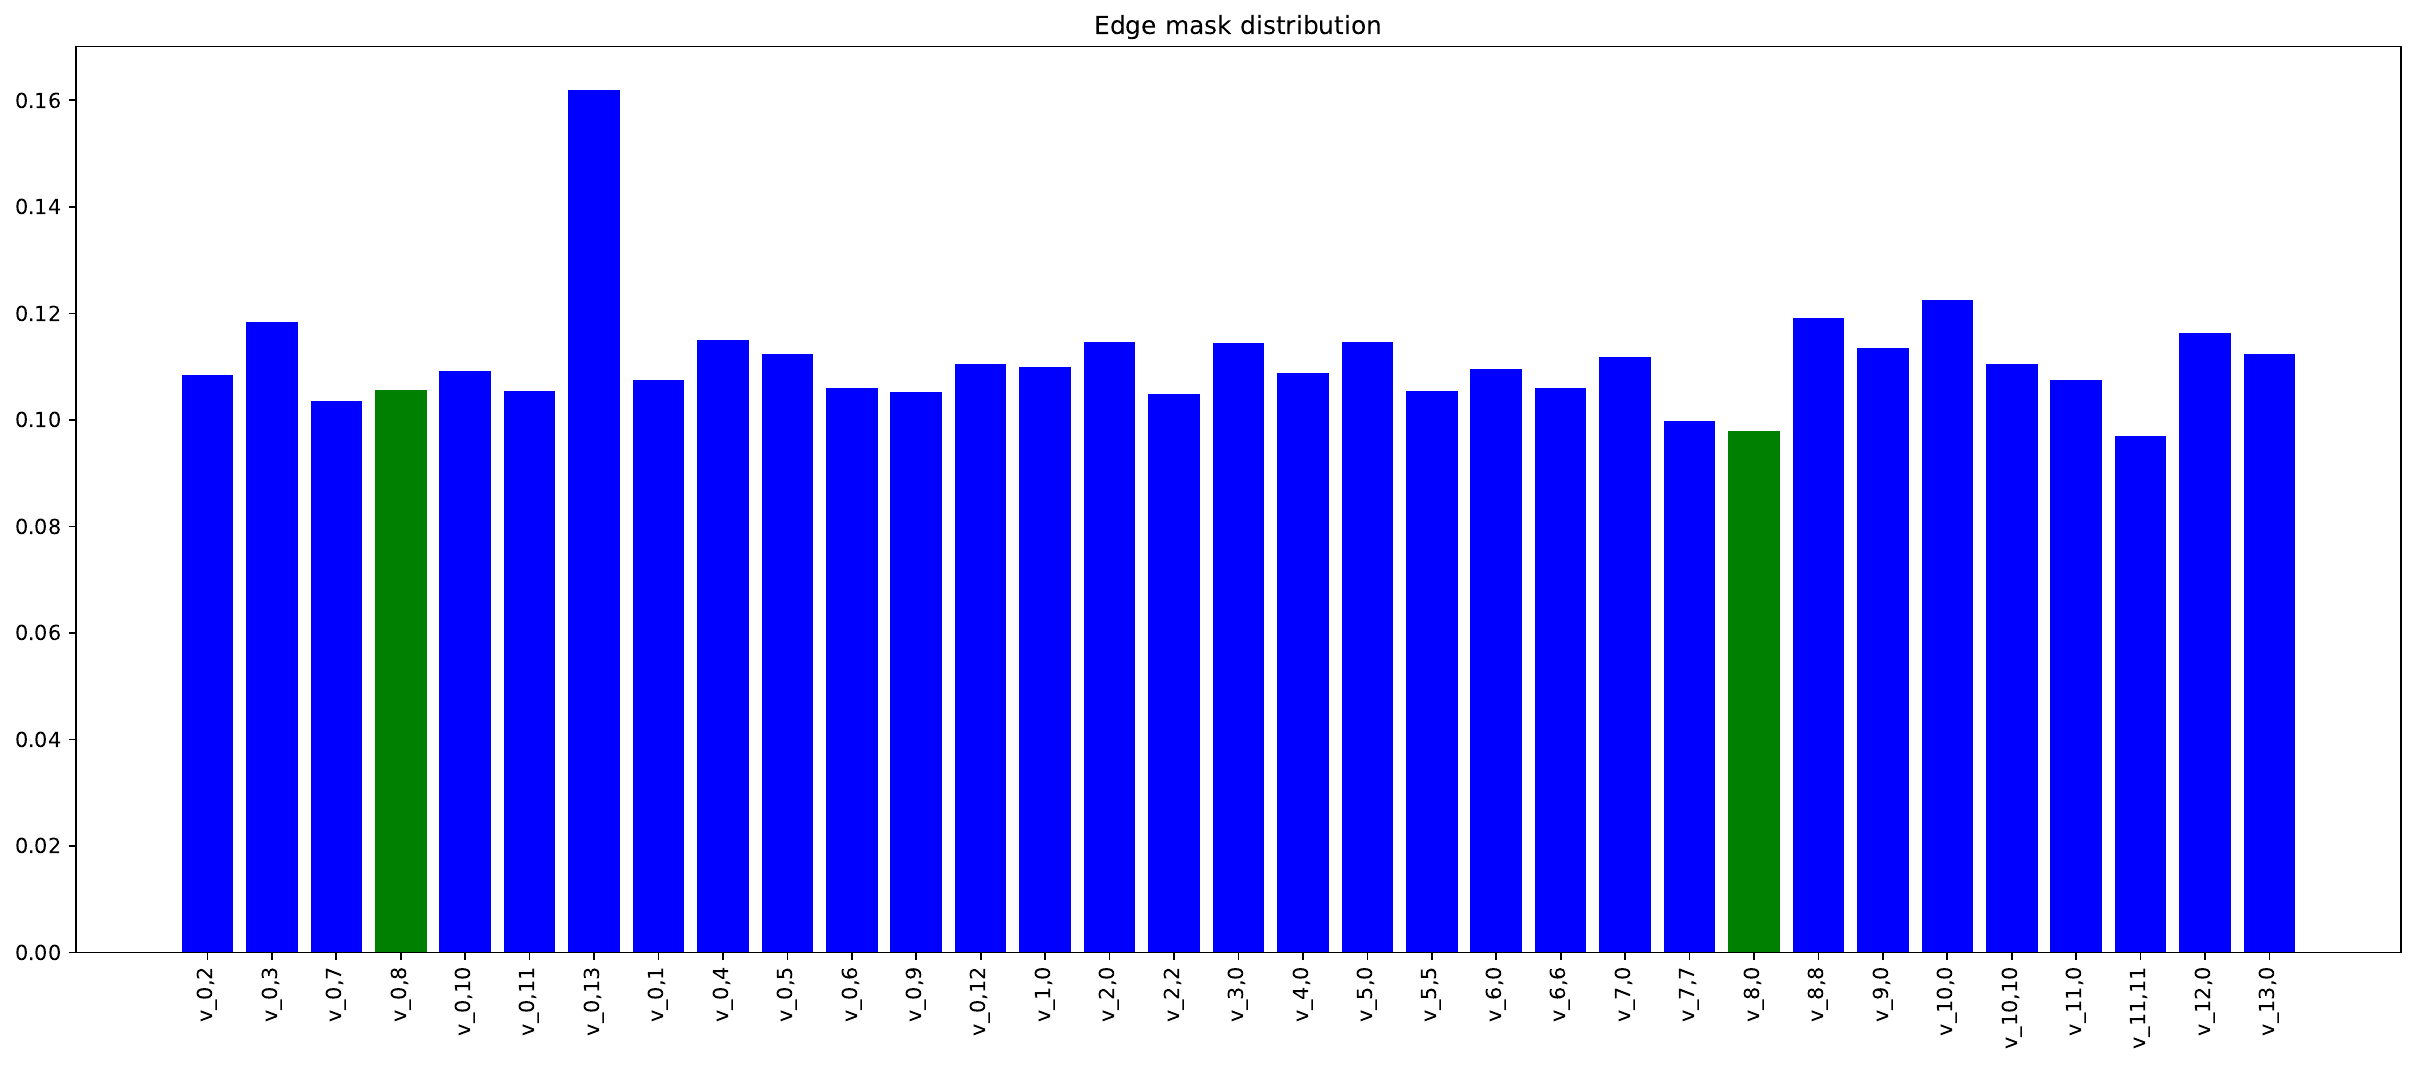
\includegraphics[scale=0.35]{EchoChamber1SubgraphEdgeMaskDistribution}
    \caption[Edge mask distribution of the subgraph provided for echo chamber example explanation.]{Edge mask distribution of the subgraph provided for echo chamber example explanation. The green bars represent the edge mask values of echo chamber connections.}
    \label{fig:EchoChamber1SubgraphEdgeMaskDistribution}
\end{figure}
Visiting back to the features we introduced, we observe that the feature $SF_7$ is captured in this explanation. To elaborate, we see that the edges to the cascade node with retweets were deemed more important by the explainer. This implies that the UPFD classifier captured an important feature for this instance. Although, this can not be clearly observed by looking at the explaining subgraph since the transparencies of the edges are not discriminative enough.\\
%Although, in order to get this interpretation, one would require a data scientist. A domain expert or an end user is likely to either misinterpret or not understand the explanation provided by GNNExplainer. Furthermore, some of the most important edges were not even included in the visualization. This certainly decreases the understandability of the explanations.\\
\textbf{The Faithfulness of Explanations.} We also analyzed the faithfulness of the explanations to the UPFD classifier. We took the explaining subgraph we provided in Fig.~\ref{fig:EchoChamberExample1Explanation_no_threshold}, restored its node features, and fed it to the UPFD classifier to see if the learned structure is still predicted as fake with high probability. In fact, the UPFD classifier predicted the subgraph as fake with $0.9915$, which is higher than the prediction probability of the original input. Overall, we say that the explaining subgraph of this instance is faithful to the UPFD classifier, and GNNExplainer can indeed reduce noise in a graph, as~\citeauthor{GNNExplainer_Ying} (\citeyear{GNNExplainer_Ying}) claim. We also observe close prediction probabilities for the original graph and the explaining subgraph in the sensitivity analysis results in Table~\ref{tab:echoChamberFeatureRemovalExperimentResults}. This further shows that this explanation is faithful for this instance.\\
\textbf{Sensitivity Analysis.} We proceed with our analysis of the echo chamber example by removing the news content and historical information of children nodes, both from the original graph and the explaining subgraph, to see their effect on the prediction. We provide the results in Table~\ref{tab:echoChamberFeatureRemovalExperimentResults}.\\
\begin{table}
    \centering
    \begin{tabular}{c | c | c}
        \textbf{Operation}            & $p_{original}$ & $p_{subgraph}$ \\
        \hline
        No change                     & 0.9912         & 0.9915         \\
        \hline
        Remove news content           & 0.8328         & 0.8018         \\
        \hline
        Remove historical information & 0.9812         & 0.9809         \\
        \hline
        Remove all node information   & 0.4940         & 0.4940         \\
    \end{tabular}
    \caption[Model prediction probabilities for input perturbation experiment.]{Model prediction probabilities for input perturbation experiment. $p_{original}$ denotes prediction probability for the original input. Analogously, $p_{subgraph}$ refers to the prediction probability for the explaining subgraph.}
    \label{tab:echoChamberFeatureRemovalExperimentResults}
\end{table}
It is trivial to observe in Table~\ref{tab:echoChamberFeatureRemovalExperimentResults} that the UPFD classifier's confidence decreases as we remove news content for the echo chamber example. Interestingly, when we remove users' historical information from all nodes except the root node, the prediction probability almost does not decrease. This suggests the UPFD classifier takes into account the news content and structural information more than the historical information. This behavior can also be observed from the UPFD classifier's architecture in Fig.~\ref{fig:UPFDClassifierArchitecture}. The skip connection and concatenation of the news content in the root node appear to be doing what is expected of it. In fact, the authors of UPFD~\parencite{UPFD_Dataset_Shu} showed that with a vanilla version of the UPFD classifier, i.e., without skip connection and concatenation, the performance drops. This finding of ours also goes in parallel with their finding. Furthermore, when we remove all node information, the UPFD classifier can no longer tell fake from real. Thus, without node information, just depending on the structure of the echo chamber example for prediction turns out to be a bad idea. We certainly need the node embeddings, at least for the news.\\
We illustrate more examples in order to understand if the statistically significant features were captured in other instances. First, it is nontrivial to look for $SF_1$ in the explanations as the tree depth will be decreased significantly. Most of the time, the tree depth in the explanations we observed was one. Thus, we skip this feature analysis. We look for the effect of feature $SF_2$ in the explanations. We compare our echo chamber example in Fig.~\ref{fig:echoChamberExample1} with a real news example in Fig.~\ref{fig:POL_RealNewsExample1}. The echo chamber example has 72 nodes, whereas the real news example has 59 nodes. Now let us observe the explanation provided for the real news instance in Fig.~\ref{fig:POL_RealNewsExample1Explanation_no_threshold}.\\
\begin{figure}
    \centering
    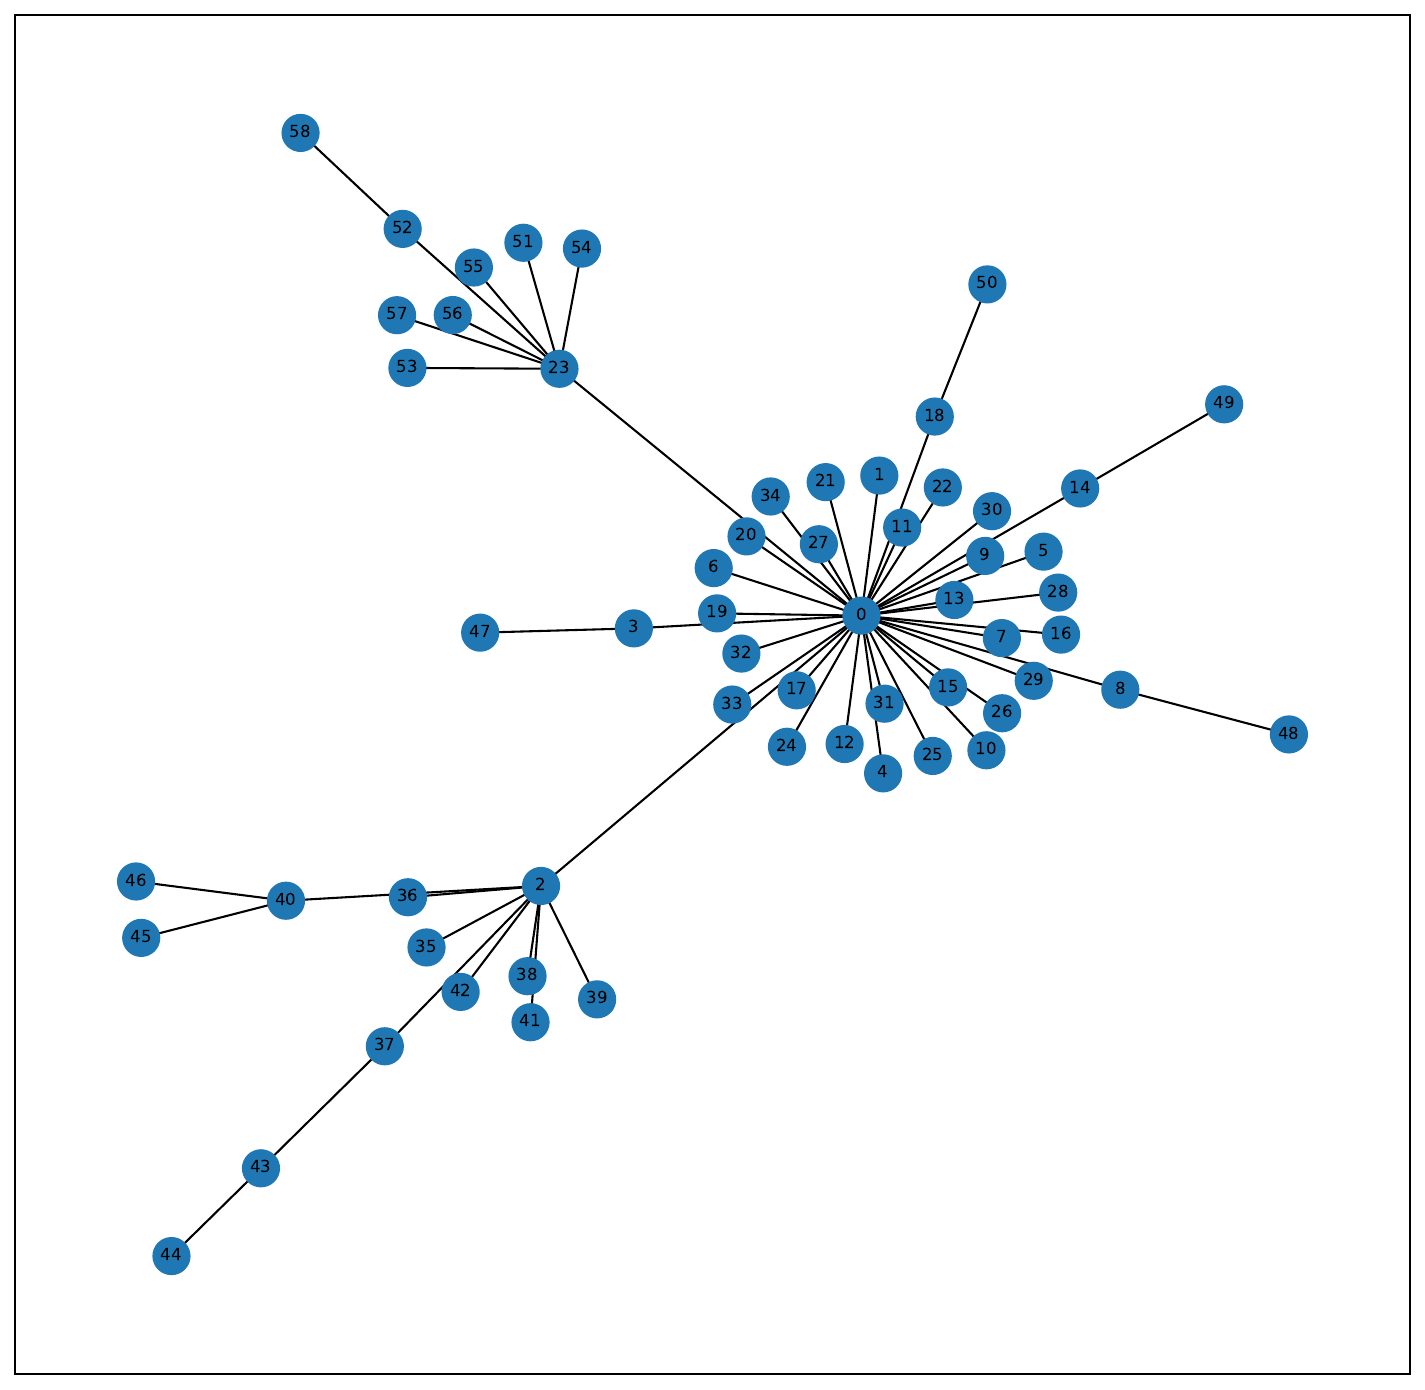
\includegraphics[scale=0.45]{POL_RealNewsExample1}
    \caption[A real news instance from UPFD-Politifact.]{A real news instance from UPFD-Politifact. We shall refer to this example as the \emph{real news example}. It was predicted as real news with probability 0.9956.}
    \label{fig:POL_RealNewsExample1}
\end{figure}
\begin{figure}
    \centering
    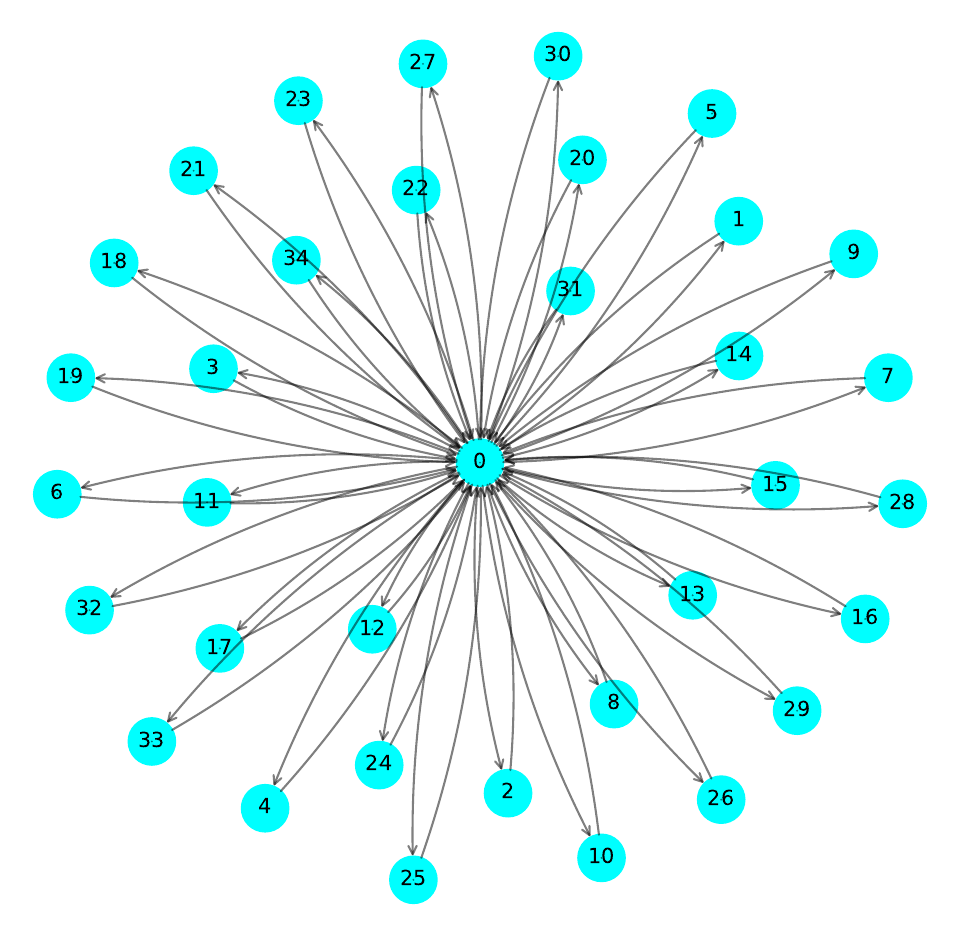
\includegraphics[scale=0.45]{POL_RealNewsExample1Explanation_no_threshold}
    \caption[Explanation of the real news example from UPFD-Politifact]{Explanation of the real news example from UPFD-Politifact. Contains 35 nodes.}
    \label{fig:POL_RealNewsExample1Explanation_no_threshold}
\end{figure}
The explaining subgraph of the real news example contains more nodes than the explaining subgraph for the echo chamber example. This might imply the effect of $SF_2$ on the explanations. In other words, explanations capture the importance of more nodes for the real news example. Although, this should be tested with other real and fake news instances to be verified. This instance has some nodes that exhibit a partial echo chamber effect. Still, we can easily observe that some of these nodes were also retweeted, a behavior not observed in the echo chamber example.\\
\textbf{Latent Space Analysis.} We apply the t-SNE~\parencite{tSNE_vanDerMaaten} function by scikit-learn~\parencite{ScikitLearn_Pedregosa} to see if GraphSAGE is able to distinguish fake and real news before its outputs are concatenated with news content in the root node and then fed to the FCN. We set the perplexity to 10, the initialization method to Principal Component Analysis (PCA), the learning rate to the \emph{auto} option, and the number of iterations to 1000, and kept the remaining parameters' default values as defined in~\cite{ScikitTSNE_scikit}. The visualization for this procedure is provided in Fig~\ref{fig:TSNE_GraphSAGE}.
\begin{figure}
    \centering
    \subfloat[UPFD-Gossipcop]{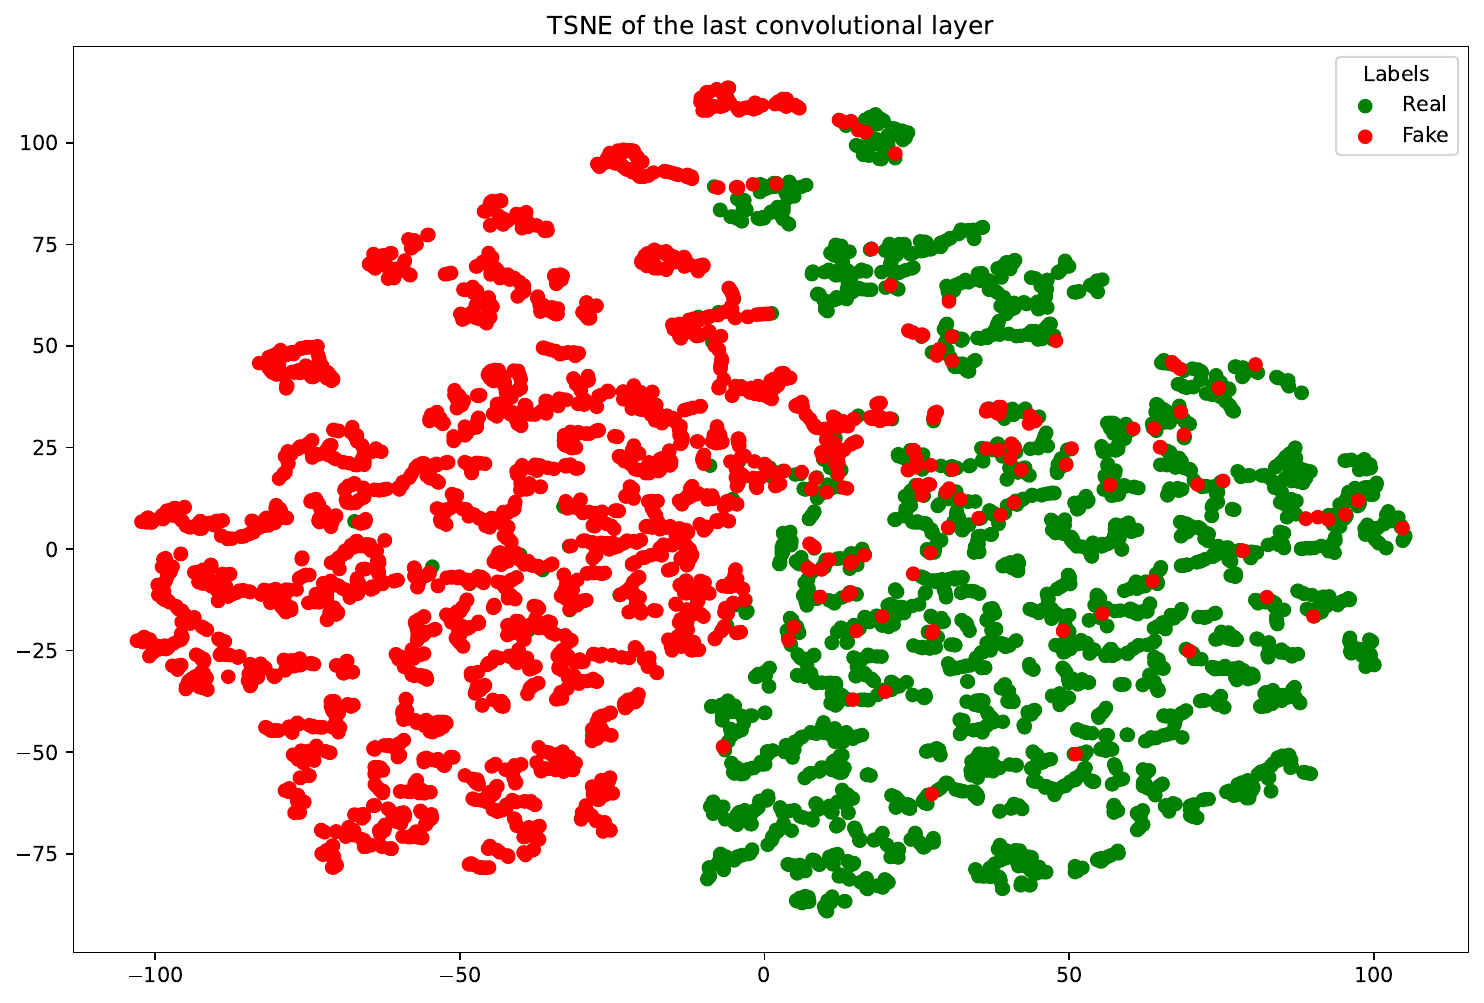
\includegraphics[width=0.45\textwidth]{TSNE_GraphSAGE_GOS.png}\label{subfig:TSNE_GraphSAGE_GOS}}
    \hfill
    \subfloat[UPFD-Politifact]{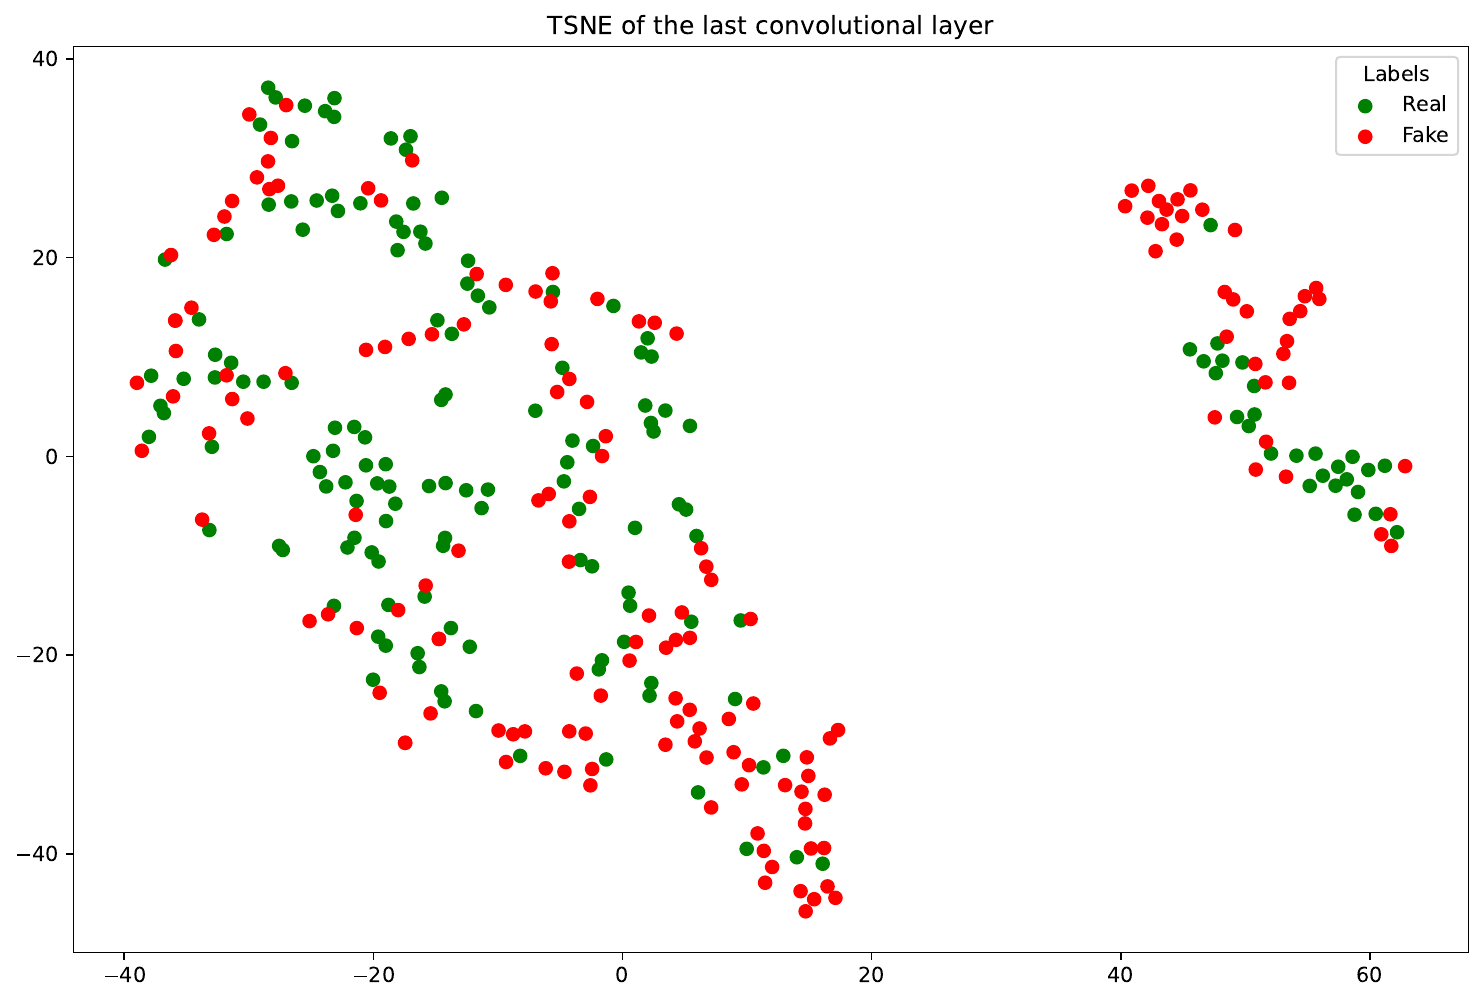
\includegraphics[width=0.45\textwidth]{TSNE_GraphSAGE_POL.png}\label{subfig:TSNE_GraphSAGE_POL}}
    \caption[t-SNE visualizations for GraphSAGE.]{t-SNE visualizations for max pooled GraphSAGE outputs on UPFD datasets.}
    \label{fig:TSNE_GraphSAGE}
\end{figure}
Clearly, GraphSAGE is able to distinguish fake and real news instances better for the UPFD-Gossipcop dataset, but it fails to make this discrimination for the UPFD-Politifact dataset. This can be due to the low amounts of instances in the UPFD-Politifact dataset.\\
\textbf{Initial Improvement Suggestions for GNNExplainer.} During our experiments, we realized that some explanations are hard to read, particularly, the ones with too many nodes and edges. Including the explanation provided in Fig.~\ref{fig:POL_RealNewsExample1Explanation_no_threshold}, it is hard to distinguish edges. In order to understand the importance of edges and simplify the explaining subgraph, we employed three simple techniques that use a threshold value. We apply this threshold value to the edge mask. This operation  sets the values less than or equal to the threshold to zero, effectively removing the corresponding edges from the explaining subgraph. The first approach is straightforward, take the maximum and the minimum value of the edge mask values. Then, set the threshold to a value less than the maximum but higher than the minimum by manual estimation, and observe the changes in the explaining subgraph as we decrease or increase the threshold value. This approach is too much manual work, so we came up with a more systematic approach. The second approach is to get the mean of all edge mask values for the current instance to get a threshold value. This way, we obtain fewer edges in our initial explanation but keep an important set of edges to understand their importance. Our third approach is to take the median of the edge mask set as a threshold. There were no big differences between the mean and median methods. However, we opted for the median method as it was able to capture more edges for small explaining subgraphs compared to the mean method. We illustrate the effect of the threshold methods on a real news instance from the UPFD-Politifact dataset in Fig~\ref{fig:POL_RealNewsExample2Explanation_with_threshold}.\\
\begin{figure}
    \centering
    \subfloat[Second real news instance from UPFD-Politifact.]{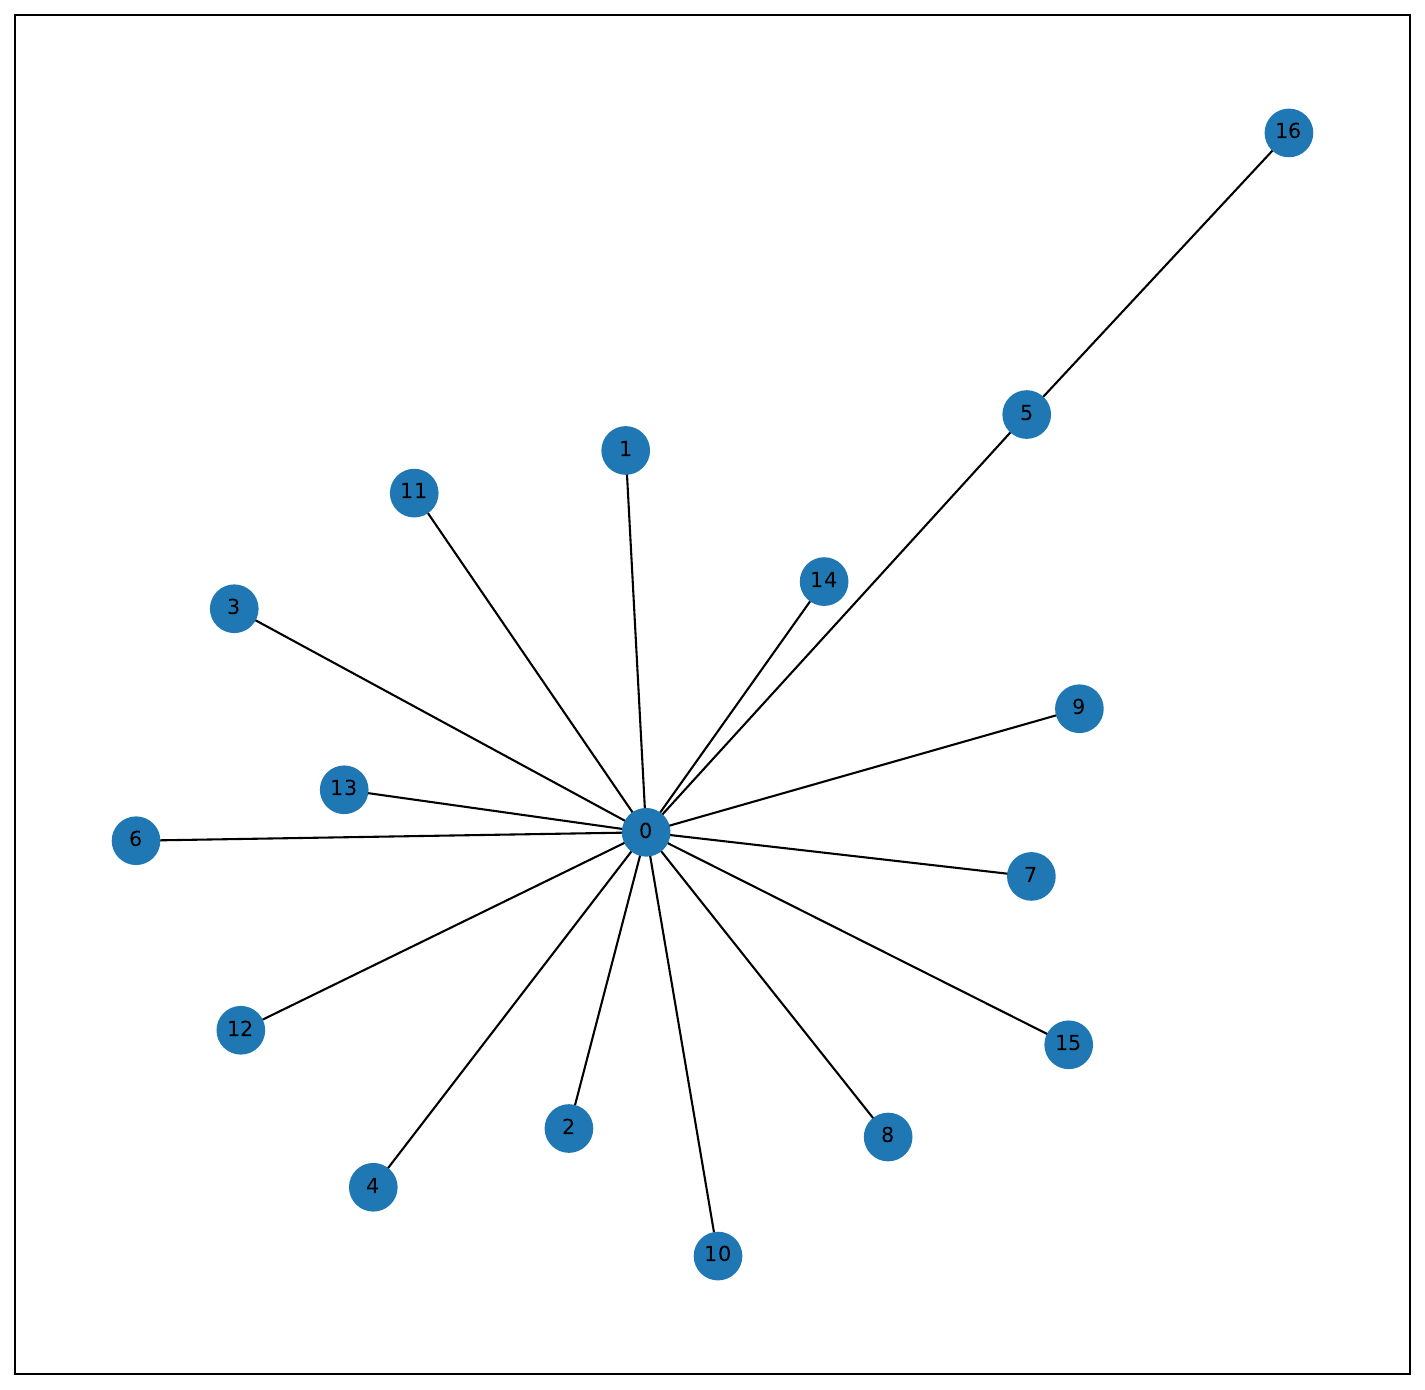
\includegraphics[width=0.45\textwidth]{POL_RealNewsExample2.png}}
    \hfill
    \subfloat[The explaining subgraph provided for the second real news instance.]{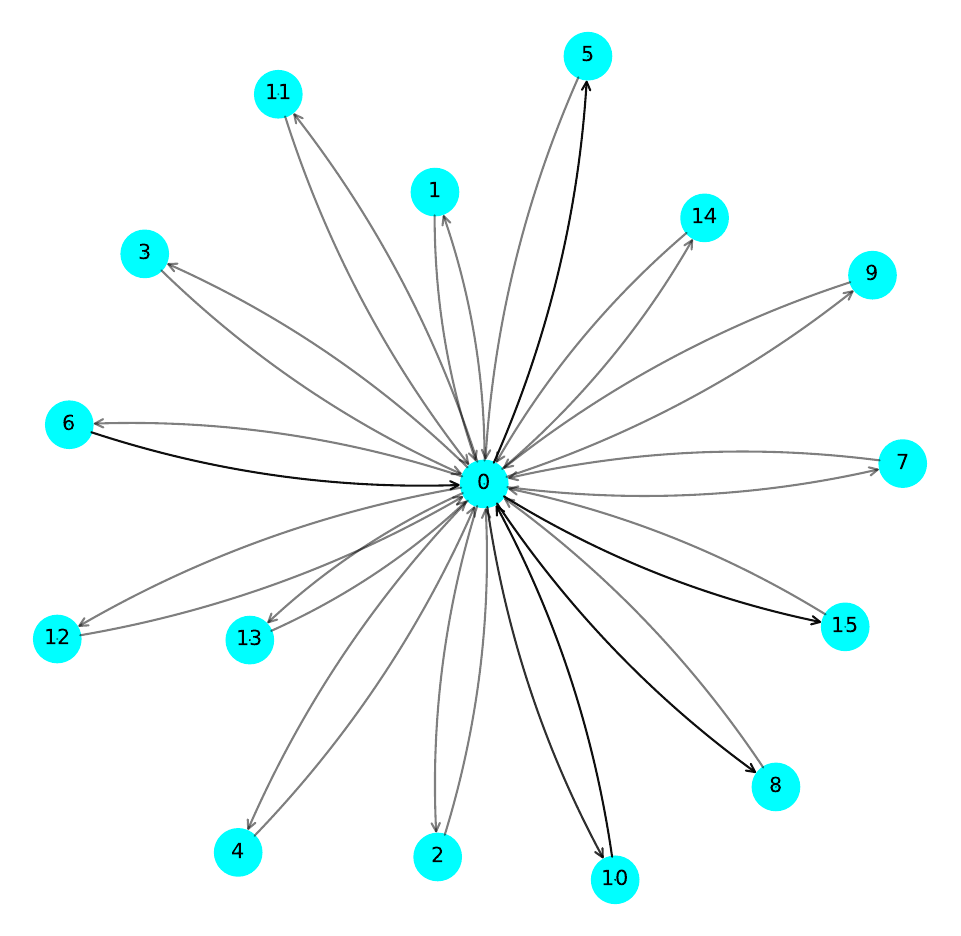
\includegraphics[width=0.45\textwidth]{POL_RealNewsExample2Explanation_no_threshold.png}}
    \hfill
    \subfloat[The explaining subgraph with median method applied.]{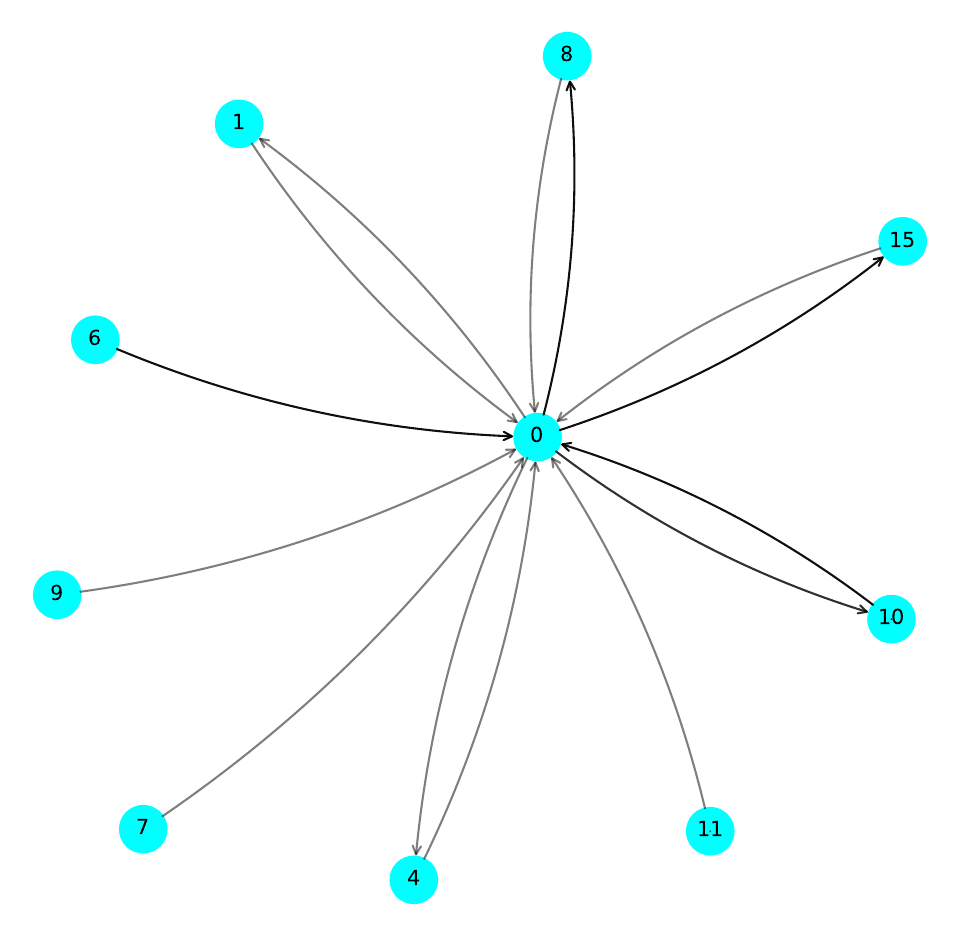
\includegraphics[width=0.45\textwidth]{POL_RealNewsExample2Explanation_with_threshold_median.png}}
    \hfill
    \subfloat[The explaining subgraph with mean method applied.]{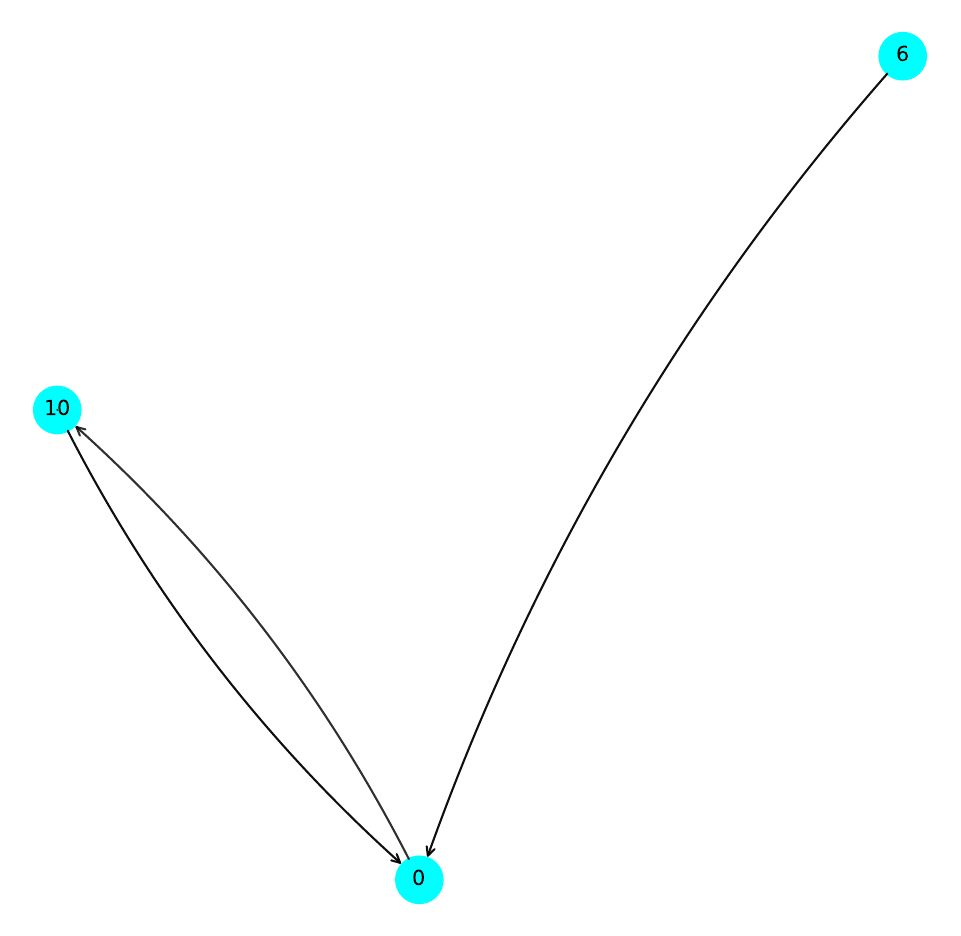
\includegraphics[width=0.45\textwidth]{POL_RealNewsExample2Explanation_with_threshold_mean.png}}
    \caption[Outputs of threshold methods for the explaining subgraph of the second real news example from UPFD-Politifact.]{Outputs of threshold methods for the explaining subgraph of the second real news example from UPFD-Politifact. We can observe that the median method provides more edges than the mean method for a relatively small explaining subgraph. Also, we can observe the importance of edges visually in the explanations. Some edges are more opaque than the other ones, this indicates that these edges are more important than the more transparent ones.}
    \label{fig:POL_RealNewsExample2Explanation_with_threshold}
\end{figure}
We can extend our method to an interactive plot in which we are able to change the threshold value dynamically. Furthermore, we can use the edge mask values provided for the edges in the subgraph to apply average and mean thresholding methods. We leave this for future work.\\
\textbf{Introducing Unseen Data.} We randomly sampled one fake news instance from the UPFD-Gossipcop dataset, which is unseen data for the UPFD classifier that was trained on the UPFD-Politifact dataset. We did not generate a new graph instance as obtaining the news piece, creating embeddings for it, and collecting its social context information is a cumbersome process without this data prepared beforehand.\\
\begin{figure}
    \centering
    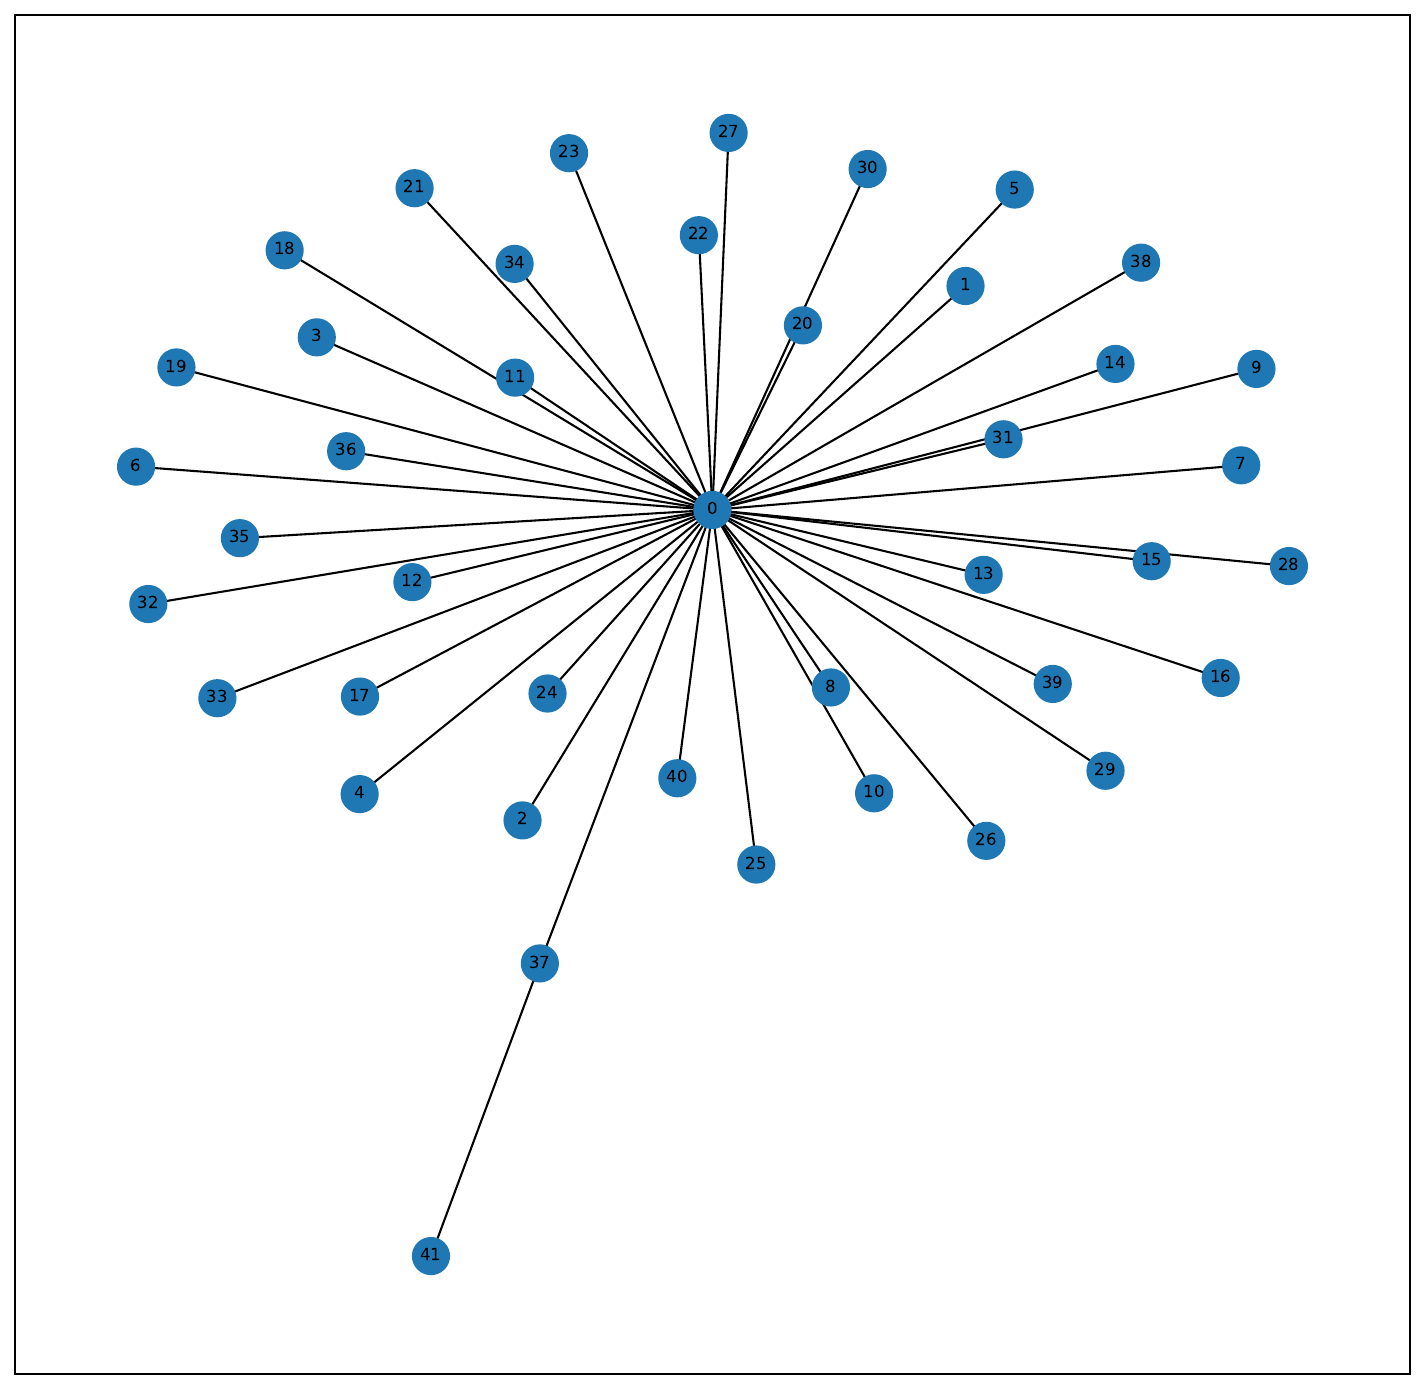
\includegraphics[scale=0.45]{GOS_FakeNewsExample1}
    \caption[A fake news example from UPFD-Gossipcop.]{A fake news example from UPFD-Gossipcop. We introduced this instance as an unseen data to the UPFD classifier, and it predicted this fake news piece as real with a probability of 0.9984.}
    \label{fig:GOS_FakeNewsExample1}
\end{figure}
Our unseen fake news example from the UPFD-Gossipcop dataset is illustrated in Fig.~\ref{fig:GOS_FakeNewsExample1}. We observe that this fake news piece does not display echo chamber patterns. In fact, structurally, it looks more like a real news piece from the UPFD-Politifact dataset. This may be why the UPFD classifier mispredicted this instance. Let us dive further into understanding this. There can be a variety of reasons. It can be because of the difference in the news style in both datasets. The UPFD-Politifact dataset houses a set of political news, whereas the UPFD-Gossipcop dataset houses a massive set of celebrity news. So, the difference in textual content could be a reason. Another reason can be the small number of training instances for the UPFD-Politifact dataset. However, we were not able to gather suggestive information from the explanation. Therefore, we did not include it. One way to understand whether the UPFD classifier responds to echo chamber structures is to create these echo chambers by adding children nodes to some of the cascade nodes and feeding this to the UPFD classifier. To test this, we added 20 nodes with no information in them and selected nodes $v_{37}$ and $v_{39}$ arbitrarily to be the spreaders. The resulting graph is illustrated in Fig.~\ref{fig:GOS_FakeNewsExample1Perturbed}.
\begin{figure}
    \centering
    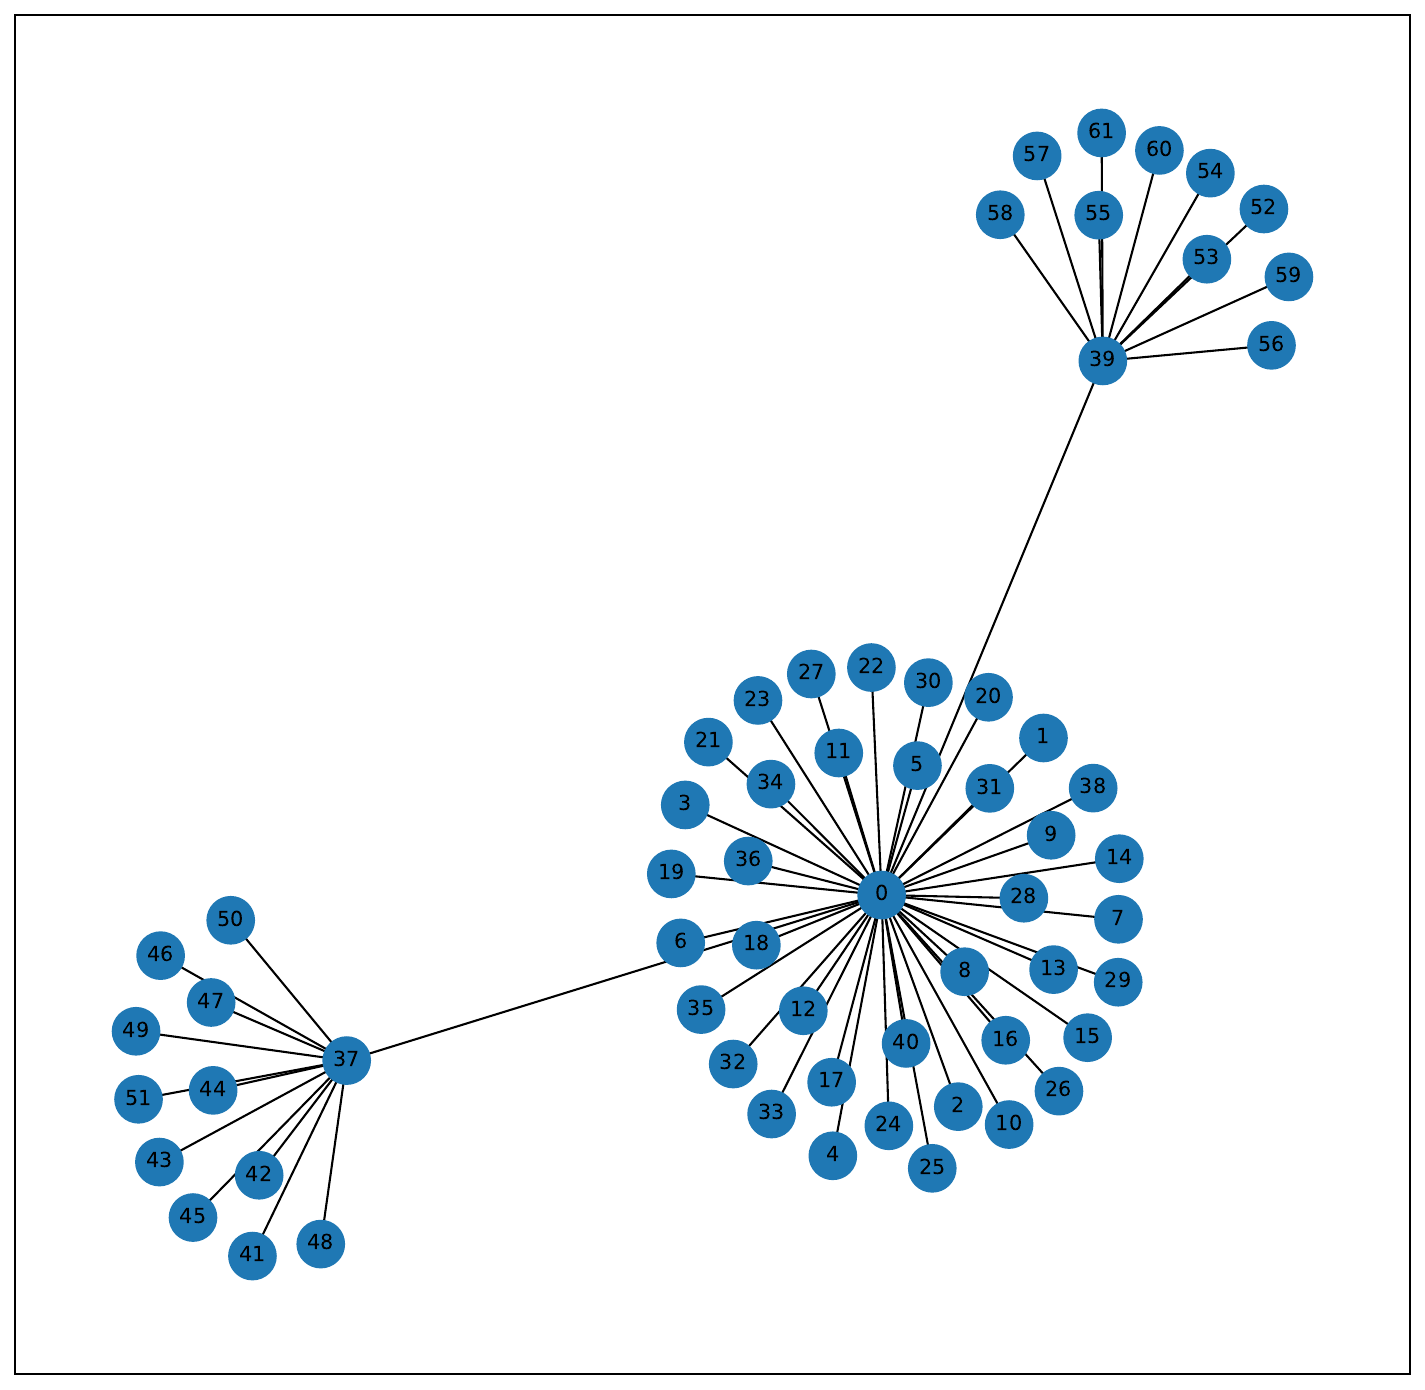
\includegraphics[scale=0.45]{GOS_FakeNewsExample1Perturbed}
    \caption[The perturbed version of the fake news example from the UPFD-Gossipcop dataset.]{The perturbed version of the fake news example from the UPFD-Gossipcop dataset. We added echo-chamber like structures to nodes $v_{37}$ and $v_{39}$.}
    \label{fig:GOS_FakeNewsExample1Perturbed}
\end{figure}
When the fed the perturbed sample to the UPFD classifier, the prediction probability of the label "fake" slightly increased. So we also sampled some historical information from a randomly obtained fake news instance that is different from the one we are analyzing. We embedded the new nodes with randomly obtained users' historical information. Then we fed this instance to the UPFD classifier, but the change in probability was too small that it could be omitted. Thus, for this instance, our experiment suggests that the existence of echo chamber structures does not increase the probability of the prediction of fake news.\\
% maybe include real news example from Gossipcop here.
\textbf{Target Audience, XAI Goals, and Final Improvement Suggestions.} Understanding the UPFD classifier's behavior locally with just a visualization is not sufficient for an end user to understand why a particular news piece was predicted as real or fake. However, given enough resources, one can reverse engineer the process in the UPFD framework, which would allow for the analysis of the node feature masks of the news content and historical information embeddings. That would increase the transparency and informativeness of the UPFD classifier. We also suggest employing interactive visualizations when working with GNNExplainer since the explanations can get very complex. Explanations produced by GNNExplainer should be investigated by a data scientist who will simplify the explanation for a domain expert or an end user. For UPFD, this simplification process can include aggregation of bidirectional edge mask values so that they can be represented as an undirected edge. Moreover, these undirected edges can be color-coded such that each color represents a value above a certain threshold which can be obtained using the methods we suggested. For example, for a big explaining subgraph, we can group the edge masks using predefined number of categories, each of which is represented by a color, then display the edges with those colors in the explaining subgraph. Also, for GNNs with language models, the node features should be easily mappable to the textual content in such a way that we can create a variation of force plots provided by the SHAP framework.\\
To sum up, we have analyzed the explanations produced by GNNExplainer for the UPFD classifier, which was trained on the UPFD-Politifact dataset. We have observed some of the statistically significant features' existence in the explanations. We have also stressed the shortcomings of GNNExplainer and suggested simple yet effective methods to reduce the complexity of an explanation. All experiments were conducted using Python 3.7~\parencite{Python_Rossum}, PyTorch 1.11.0~\parencite{PyTorch_Paszke}, and PyTorch Geometric 2.0.4~\parencite{PyTorchGeometric_Fey}. All visualizations were obtained through the use of NetworkX 2.6.3~\parencite{NetworkX_Hagberg}, and Matplotlib 3.5.1~\parencite{Matplotlib_Hunter}. The detailed library usage and the implementation of all models are provided in our GitHub repository~\footnote{\url{https://github.com/sersery35/Explainability_of_FND_Models/tree/main/GNNFakeNews}}.